%\documentclass[twoside]{pwrthesis}
\documentclass[twoside]{iisthesis}
% ---

\usepackage{polski}
\usepackage[utf8]{inputenc}
\usepackage{amsmath}
\usepackage{tocloft}
\usepackage{listings}
\usepackage{algorithm}
\usepackage{algorithmic}
\usepackage{subcaption}
\usepackage{mathtools}
\usepackage{graphicx}
\usepackage[colorinlistoftodos,prependcaption,textsize=tiny]{todonotes}
\usepackage{url}
\usepackage{pgfplots, pgfplotstable}
\pgfplotsset{compat=1.13}
\usepackage{array,tabularx}
\selectlanguage{polish}
% Dodane przeze mnie d
\usepackage{fancyvrb} % dla srodowiska Verbatim
\usepackage{color}
\usepackage{lscape}
\usepackage{longtable}

\let\lll\undefined
\usepackage{amssymb}

\hypersetup{
    colorlinks,
    linkcolor={black!50!black},
    citecolor={black!50!black},
    urlcolor={black!80!black}
}

\definecolor{gray}{rgb}{0.4,0.4,0.4}
\definecolor{darkblue}{rgb}{0.0,0.0,0.6}
\definecolor{cyan}{rgb}{0.0,0.6,0.6}

\lstset{
  basicstyle=\ttfamily,
  columns=fullflexible,
  showstringspaces=false,
  commentstyle=\color{gray}\upshape
}

\lstdefinelanguage{XML}
{
  morestring=[b]",
  morestring=[s]{>}{<},
  morecomment=[s]{<?}{?>},
  stringstyle=\color{black},
  identifierstyle=\color{darkblue},
  keywordstyle=\color{cyan},
  morekeywords={xmlns,version,type}% list your attributes here
}

\lstset{
  language=XML,
   literate={ć}{{\'c}}1
}
\renewcommand*{\lstlistingname}{Kod źródłowy}
% definicje kolorow
\definecolor{ciemnoSzary}{rgb}{0.15,0.15,0.15}
\definecolor{szary}{rgb}{0.5,0.5,0.5}
\definecolor{jasnoSzary}{rgb}{0.2,0.2,0.2}

% Konfiguracja verbatima
\fvset{
	frame=single,
	numbers=left,
	fontsize=\footnotesize,
	numbersep=12pt,
%	framerule=.5mm,
	rulecolor=\color{ciemnoSzary},
%	fillcolor=\color{jasnoSzary},
	framesep=4pt,
	stepnumber=1,
	numberblanklines=false,
	tabsize=2,
%	formatcom=\color{szary}
}
\newcommand{\listequationsname}{Spis wzorów}
\newcommand{\equationcaption}[1]{\begin{flushright}\emph{#1}\end{flushright}}
\newcommand{\rightcaption}[1]{\begin{flushright}\emph{#1}\end{flushright}}
\newlistof{myequations}{equ}{\listequationsname}
\newcommand{\myequations}[1]{%
\addcontentsline{equ}{myequations}{\protect\numberline{\theequation}#1}\par}

\newcommand{\listofmyalgorithmsname}{Spis algorytmów}
\newlistof{myalgorithm}{algo}{\listofmyalgorithmsname}
\newcommand{\myalgorithm}[1]{%
\addcontentsline{algo}{myalgorithm}{\protect\numberline{\thealgorithm}#1}\par}


\newcommand{\listofmyfiguresname}{Spis rysunków}
\newlistof{myfigure}{figu}{\listofmyfiguresname}
\newcommand{\myfigure}[1]{%
\addcontentsline{figu}{myfigure}{\protect\numberline{\thefigure}#1}\par}

\floatname{algorithm}{Algorytm}

\newtheorem{mydef}{Definicja}

%tables
\setlength{\tabcolsep}{0.5em} % for the horizontal padding
{\renewcommand{\arraystretch}{1.25}% for the vertical padding

\newcolumntype{R}[1]{>{\raggedleft\let\newline\\\arraybackslash\hspace{0pt}}m{#1}}

\begin{document}


\newcommand{\resultChart}[7][140]{
\def\dataS{{#2}}
	\begin{figure}[H]
	
\centering

\begin{center}
\begin{tikzpicture}
 
\begin{axis}[
ybar,
bar width=20,
legend style={at={(0.5,-0.25)},
anchor=north,legend columns=-1},
ylabel={Wartość miary},
symbolic x coords={\dataS},
xtick=data,
height=  {#1},
width=0.8\textwidth,
ymin=0, ytick={0,0.5,1},
ymax=1.5,
nodes near coords,
nodes near coords align={vertical},
]
\addplot coordinates { (\dataS,{#3}) };
\addplot coordinates {(\dataS,{#4}) };
\addplot coordinates { (\dataS,{#5}) };
\legend{Recall,Precission,F1-Score}
\end{axis}
\end{tikzpicture}
\end{center}
\caption{{#6}}
\myfigure{{#6}}
\label{{#7}}
\end{figure}
}


\pgfkeys{/pgf/number format/use comma}
\pgfkeys{/pgf/number format/.cd, set thousands separator={}}%
\nocite{*}
\title{ TITLE }
\titleEN{ TITLE EN}
\shortTitle{SHORT TITLE}
\author{Katatzyna Biernat }
\advisor{dr inż. Bernadetta Maleszka}
\instituteLogo{logos/pwr}
\slowaKluczowe{KEYWORDS}

\date{\number\the\year}

% Wstawienie abstractu pracy
	%\input {abstract}

\abstractSH{SHORT ABSTRACT}

\abstractPL{
ABSTRACT PL
}
\abstractEN{
ABSTRACT EN
}

\maketitle
\textpages


\graphicspath{ {img/} }
\DeclareGraphicsExtensions{.pdf,.png,.jpg,.svg}

  \listoftodos

\todo{ujednolicić terminologię content-based/collaborative. Która wersja?}

 \chapter{Wstęp}
 \shortTitle{Wstęp}
	 Wraz z rozwojem Internetu zmienił się sposób dostępu do informacji. Kiedyś to użytkownik musiał walczyć pozyskanie wiedzy; dzisiaj to informacje walczą u uwagę użytkowników. W świecie zalanym wiadomościami koniecznym wydaje się być zastosowanie filtra, który odsieje interesującą  i wartościową zawartość od tej niechcianej. Pomocne okazują się zautomatyzowane mechanizmy rekomendacji.
	 
	 Jednakże sama idea rekomendacji nie jest niczym nowym. Co więcej, zjawisko to możemy zaobserwować w naturze -- na przykład wśród mrówek, które podążają wyznaczoną (rekomendowaną) ścieżką feromonową w poszukiwaniu pożywienia.
	 
	 Ludzie od niepamiętnych czasów posiłkowali się opiniami innych, aby ułatwić sobie dokonanie wyboru, od najbliższego grona znajomych do ekspertów i autorytetów.
	 
	 Wraz z rozwojem nauk informatycznych problem rekomendacji stał się problemem interesującym badaczy. Za pierwszy system rekomendacji uznaje się \textit{Tapestry} stworzony w laboratoriach Xerox Palo Alto Research Center w 1992 roku. Motywacją było odfiltrowanie rosnącej liczby niechcianej poczty elektronicznej \cite{id:FromTapestryToSVD}.
	 
	 Wkrótce później idea ta została rozszerzona przez takich graczy jak Amazon, Google, Pandora, Netflix, Youtube, Yahoo etc. aż do formy, jaką znamy dzisiaj: systemu, który sugeruje użytkownikom produkty, filmy, muzykę, strony internetowe na podstawie ich aktywności w sieci \cite{id:EvolutionOfRecommenderSystems}. 
	 
	 Wielkie koncerny internetowe stale poprawiają jakość swoich algorytmów rekomendacji. Najlepszym przykładem jest tutaj Netflix, który w październiku 2006 zorganizował ogólnodostępny konkurs na najlepszy algorytm. Zadaniem uczestników było ulepszenie algorytmu Cinematch. Już po siedmiu dniach od ogłoszenia konkursu trzy zespoły zdołały poprawić wynik Cinematch o 1.06\% \cite{id:NetflixPrize,id:NetflixPrizeRankings}. 18 września 2009 Netflix ogłosił, że zespół BellKor's Pragmatic Chaos poprawił Cinematch o 10,06\% osiągając wynik $RMSE = 0.8567$. Tym samym wygrał nagrodę w wysokości \$1,000,000 i zakończył konkurs \cite{id:NetflixPrize2,id:NetflixPrizeRules}.
	 
	 Systemy rekomendacji ulepszane są nieustannie, o czym świadczy chociażby organizowana rokrocznie konferencja\textit{ ACM International Conference on Recommender Systems}. Tematyka ta poruszana jest także na konferencjach \textit{European Conference on Information Retrieval}, \textit{European Conference on Machine Learning and Principles and Practice of Knowledge Discovery in Databases} i wielu innych. Mimo dużego stopnia zaawansowania wciąż istnieje pole manewru do ulepszania algorytmów rekomendacji i co za tym idzie zwiększanie zadowolenia użytkowników, które z kolei prowadzi do osiągania korzyści biznesowych.
	 
	 Celem pracy jest opracowanie i zbudowanie hybrydowego algorytmu rekomendacji. Składowymi docelowego algorytmu są metody kolaboratywnego filtrowania oraz metody filtrowania z analizą treści.  
	 
	 \todo{CEL PRACY: trzeba rozszerzyć opis, w szczególności o to, co jest nowego i czym różni się od innych już istniejących algorytmów}
	 
	 W kolejnych rozdziałach przedstawione są istniejące oraz proponowane ulepszenia, które pozwalają na jeszcze lepsze dopasowanie wyników rekomendacji do oczekiwań użytkowników. 
	 
	 \todo{streszczenie spisu treści}
	 
 
 \chapter{Przegląd istniejących rozwiązań}
 \shortTitle{Przegląd istniejących rozwiązań}
	 Tradycyjnie wyróżniamy następujące techniki rekomendacji: 
	 
	 \begin{itemize}
	 	\item \textbf{filtrowanie w oparciu o zawartość} (ang. \textit{content-based filtering}), technika koncentrująca się na atrybutach elementów. Użytkownikowi rekomendowane są elementy, które podobne są do tych wybieranych przez niego w przeszłości;
	 	\item \textbf{filtrowanie kolaboratywne} (ang. \textit{collaborative filtering}), technika polegająca na odnajdywaniu użytkowników o podobnych gustach i sugerowaniu lubianych przez nich elementów aktualnie aktywnemu użytkownikowi;
	 	\item \textbf{filtrowanie demograficzne} (ang. \textit{demographic filtering}), technika koncentrująca się na sugerowaniu aktywnemu użytkownikowi elementów popularnych pośród użytkowników z tej samej okolicy bądź w podobnym przedziale wiekowym;
	 	\item \textbf{filtrowanie z analizą domeny wiedzy} (ang. \textit{knowledge-based filtering}), technika dobierająca kolejne elementy na podstawie określonej domeny wiedzy na temat tego, jak dany element spełnia potrzeby i preferencje użytkownika;	
	 	\item \textbf{filtrowanie z analizą społecznościową} (ang. \textit{community-based filtering}), technika dobierająca rekomendacje dla użytkownika w zależności od preferencji innych użytkowników z jego sieci społecznościowej. W myśl zasady ,,powiedz mi kim są twoi przyjaciele a powiem ci kim jesteś'';
	 	\item \textbf{hybrydowe systemy rekomendacji} to kombinacja dowolnych powyższych technik.
	 \end{itemize}
	 
	 Każda z tych technik ma swoje wady i zalety w zależności od kontekstu, w którym ma być stosowana \cite{id:IntroductionToRecommenderSystemsHandbook}. 
	 
	 \todo{krótka wzmianka o tym, że w kolejnych podrozdziałach będą opisane wybrane techniki - te, które będą wykorzystywane w Pani systemie}
	 
	 \section{Filtrowanie w oparciu o zawartość}
	 
	 Filtrowanie content-based opiera się na cechach elementów w systemie. Rekomendowane są obiekty, które podobne są do tych pozytywnie ocenionych wcześniej przez użytkownika \cite{id:huynh2012modeling}. W zależności od domeny pod uwagę mogą być brane słowa kluczowe, cechy takie jak rok wydania, reżyser, autor, kompozytor, gatunek itp.
	 
	 \subsection{Metody tworzenia profilu użytkownika}
	 \label{ss:metody_tworzenia_profilu_uzytkownika}
	 
	 Profil użytkownika może być tworzony na dwa sposoby. Jeżeli użytkownik jawnie pozostawia informacje można mówić o podejściu aktywnym (explicit feedback). Do takich informacji należą: ocena konkretnych elementów, tzw. łapka \todo{kolokwializm - jak poprawić?} w górę lub w dół, komentarz itp. 
	 
	 Jednakże nawet jeżeli użytkownik nie jest skory do zostawiania tego typu śladów, to i tak można wiele na jego temat wywnioskować korzystając z podejścia pasywnego (ang. \textit{implicit feedback}). System bierze wówczas pod uwagę aktywność użytkownika taką jak: historia zakupów, historia przeglądarki a nawet ruchy myszką. W przypadku serwisu z muzyką czy filmem cenną informacją będzie fakt, czy użytkownik wysłuchał lub obejrzał dany materiał do końca czy też wyłączył go po paru sekundach \cite{id:AdvancesInCollaborativeFiltering,id:ContentBasedRecommenderSystemsState}.
	 
	 \subsection{Zalety podejścia content-based}
	 
	 Do zalet filtrowania w oparciu o zawartość należy niezależność użytkownika. Podczas budowania rekomendacji brany pod uwagę jest tylko jego profil; aktywność innych aktorów w systemie nie wpływa na wynik końcowy. \todo{ktoś może Pani zarzucić, że to wada, bo nie korzystamy z informacji, które są dostępne} Inną przewagą jest przejrzystość -- każda propozycja jest w pełni uzasadniona, gdyż opiera się na działaniach użytkownika w przeszłości (podczas gdy w przypadku filtrowania kolaboratywnego mamy do czynienia z czarną skrzynką \todo{tutaj albo trzeba rozwinąć myśl, albo nie pisać w ogóle o czarnych skrzynkach}). Ponadto, tego typu algorytm ma możliwość zaproponowania elementu, który nie był nigdy wcześniej oceniany przez nikogo. Zapobiega to zjawisku długiego ogona	 \cite{id:ContentBasedRecommenderSystemsState}.
	 
	 \subsection{Wady podejścia content-based}
	 Aby rekomendacja była skuteczna użytkownik powinien ocenić jak najwięcej elementów. Problematyczni są zatem użytkownicy, którzy dopiero co dołączyli do serwisu oraz tacy, którzy nie są aktywni i rzadko zostawiają po sobie ślad \cite{id:MaleszkaMianowskaNguyenmethod}.
	 
	 Podejście content-based jest podatne na pułapkę tzw. bańki informacyjnej. Jeżeli w systemie rekomendującym produkcje kinowe użytkownik do tej pory oceniał jedynie filmy akcji, to mało prawdopodobne jest, że algorytm zaproponuje mu ciekawy dramat obyczajowy. Nowe propozycje nie są zaskakujące \cite{id:ContentBasedRecommenderSystemsState}.
	 
	 \section{Filtrowanie kolaboratywne}
	 
	 Filtrowanie kolaboratywne opiera się na założeniu, że ludzie o zbliżonym guście dokonują podobnych wyborów. Użytkownicy o zbliżonym guście to osoby, które oceniły konkretne elementy w podobny sposób \cite{id:IntroductionToRecommenderSystemsHandbook, id:CollaborativeFilteringRecommenderSystems, id:huynh2012modeling}. 
	 
	 W przypadku filtrowania kolaboratywnego można wyróżnić dwa główne podejścia: oparte o regułę sąsiedztwa (ang. \textit{neighborhood}) oraz oparte o model (ang. \textit{model-based}), wykorzystujące modele ukrytych parametrów \cite{id:AdvancesInCollaborativeFiltering,koren2009matrix}. 
	 
	 \begin{figure}[!ht] 
	 	\centering
	 	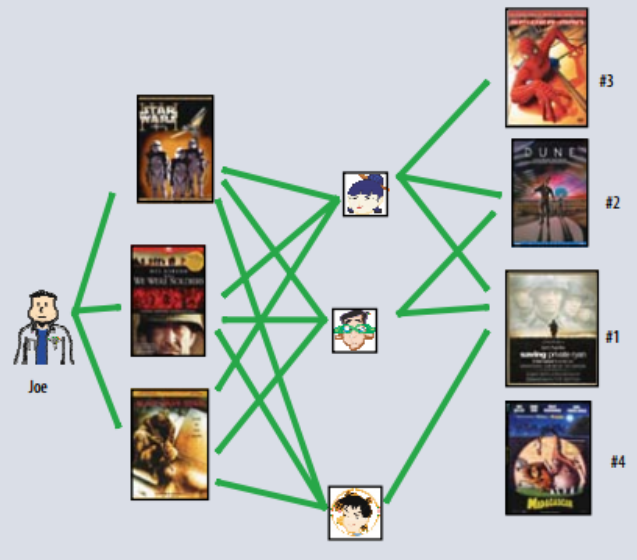
\includegraphics[width=0.7\textwidth]{cf}
	 	\caption{Filtrowanie kolaboratywne metodą sąsiedztwa,  zorientowane na użytkownika \protect\cite{koren2009matrix}.}
	 	\label{fig:cf}
	 \end{figure}
	 
	 Filtrowanie w oparciu o regułę sąsiedztwa koncentruje się na związkach element-element bądź użytkownik-użytkownik \cite{id:AdvancesInCollaborativeFiltering}.
	 Rysunek \ref{fig:cf} pokazuje regułę sąsiedztwa skoncentrowaną na relacji użytkownik-użytkownik. Joe ocenił trzy filmy. System odnajduje innych użytkowników, którzy ocenili te trzy pozycje podobnie jak Joe. Każdy z nich pozytywnie ocenił film ,,Saving Private Ryan", zatem jest to pierwsza rekomendacja dla Joe. 
	 
	  \begin{figure}[!ht] 
	  	\centering
	  	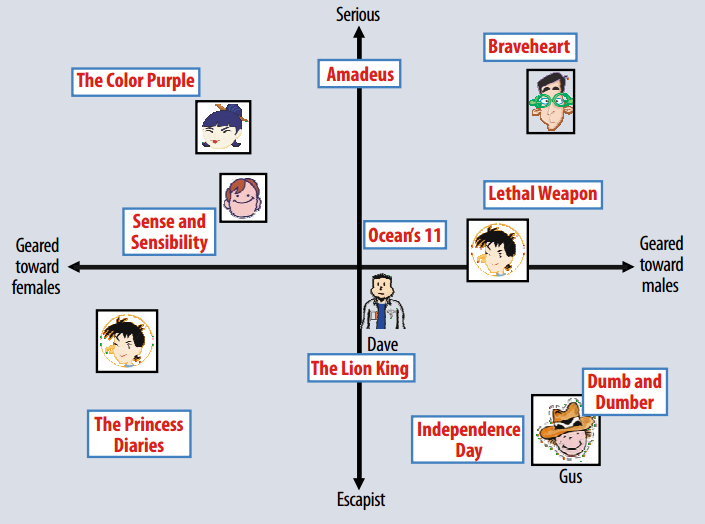
\includegraphics[width=0.7\textwidth]{cf2}
	  	\caption{Filtrowanie kolaboratywne z wykorzystaniem modelu ukrytych parametrów \protect\cite{koren2009matrix}.}
	  	\label{fig:cf2}
	  \end{figure}
	 
	 Ideą podejścia model--based \todo{która wersja językowa jest lepsza?} jest zbadanie i modelowanie zależności element--użytkownik wraz z czynnikami reprezentującymi ukryte własności elementów i użytkowników. Taki model jest następnie uczony przy użyciu dostępnych danych. W rezultacie można z niego odczytać przewidywaną ocenę elementu dla konkretnego użytkownika \cite{id:ComprehensiveSurveyOfNeighborhoodBasedRecommendationMethods, id:AdvancesInCollaborativeFiltering}.
	 
	 Rysunek \ref{fig:cf2} pokazuje w sposób uproszczony podejście oparte o model. W układzie współrzędnym oznaczeni są użytkownicy wedle swoich preferencji oraz konkretnych cech (np. płeć) a także filmy, które stanowią odpowiedź na dany zestaw preferencji/cech \cite{koren2009matrix}. 
	 
	 \subsection{Zalety filtrowania kolaboratywnego}
	 
	 \todo{Zalety filtrowania kolaboratywnego}
	 
	 \subsection{Wady filtrowania kolaboratywnego}
	 
	 Jednym z problemów klasycznego podejścia do kolaboratywnego filtrowania jest brak uwzględnienia dynamiki zmian w gustach użytkowników. Ten sam użytkownik na przestrzeni kilku lat lub miesięcy może zupełnie inaczej ocenić ten sam film bądź piosenkę. Rozwiązaniem jest dodanie czynnika czasu podczas obliczania wag kolejnych ocen. \cite{id:NewRecommentationAlgoritmBasedOnSocialNetwork,id:NextSongRecommendationWithTemporalDynamics,koren2009matrix}.
	 
	 Innym problemem jest tzw. zimny start (ang. \textit{cold start}). Polega on na tym, że nowi użytkownicy w systemie ocenili zbyt mało elementów, aby można było zbudować dla nich dobre rekomendacje \cite{id:RubensRecSysHB2010,id:zhang2015hybrid}.
	 
	 Powszechnym zjawiskiem jest tzw. efekt długiego ogona. Rysunek \ref{fig:longtail} przedstawia jak rozkłada się procentowa ilość ocen danych elementów w zależności od ich popularności. Jeżeli algorytm rekomendacji nie wspiera mniej popularnych elementów, to istnieje ryzyko, że użytkownicy nie otrzymają możliwości eksplorowania nowych, niszowych materiałów \cite{id:celma2010music,id:RubensRecSysHB2010}.
	 
  \begin{figure}[!ht] 
 	  	\centering
 	  	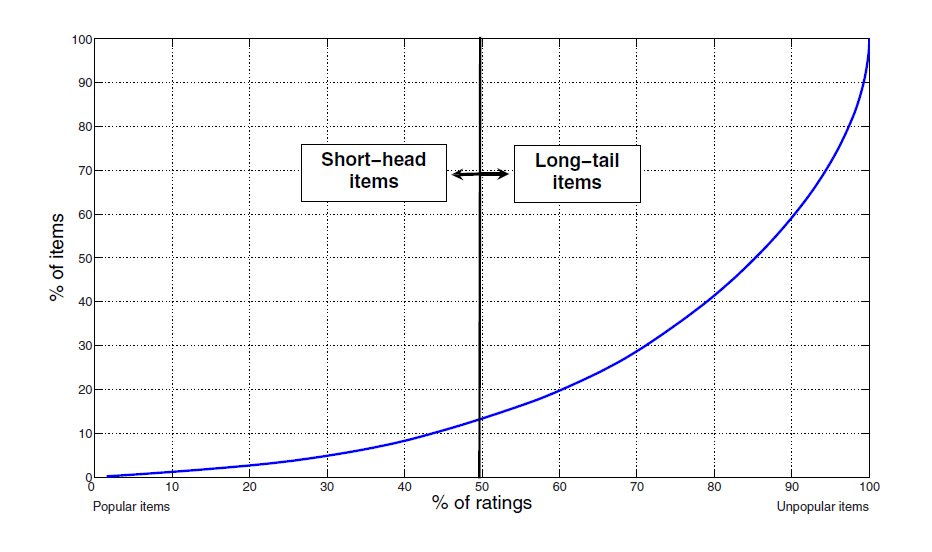
\includegraphics[width=0.7\textwidth]{longtail}
 	  	\caption{Problem długiego ogona: 50\% ocen dotyczy 10-12\% najpopularniejszych elementów w systemie \protect\cite{id:RubensRecSysHB2010}.}
 	  	\label{fig:longtail}
  \end{figure}
	 
	 Systemy rekomendacji wykorzystujące filtrowanie kolaboratywne nie są skalowalne. Złożoność rośnie proporcjonalnie do ilości użytkowników i elementów. Wielkie koncerny internetowe takie jak Twitter wykorzystają klastry i maszyny z bardzo dużą pamięcią aby zachować płynność działania serwisu \cite{id:gupta2013wtf}.
	 
	 \subsection{Algorytmy hybrydowe}
	 \todo{opisać istniejące algorytmy hybrydowe i na czym polegają etc}
	 
	 \section{Popularne serwisy wykorzystujące algorytmy rekomendacji}
	 
		W przeciągu ostatnich lat algorytmy rekomendacji zagościły na bardzo wielu popularnych serwisach internetowych z różnych domen. Poniższa lista prezentuje garstkę wybranych stron. 
	 
		 \subsection{Rekomendacja muzyki}
	 
		 \begin{itemize}
		 	\item \textbf{YouTube} -- serwis powstały w 2005 roku, pozwalający na bezpłatne umieszczanie, odtwarzanie, ocenianie i komentowanie filmów. Od 2006 roku przejęty przez Google. YouTube buduje profil użytkownika w oparciu o jego aktywność w serwisie. Brane pod uwagę są polubienia (łapka \todo{poprawić kolokwializm} w górę), subskrypcje, udostępnianie a także informacje czy użytkownik obejrzał film do końca czy tylko pewien jego procent. Techniki rekomendacji stosowane przez serwis to przede wszystkim wydobywanie reguł asocjacyjnych i licznik wspólnych odwiedzin danego wideo w czasie trwania pojedynczej sesji \cite{id:TheYouTubeVideoRecommendationSystem}. 
		 	\item \textbf{LastFM } -- internetowa radiostacja oferująca rozbudowany mechanizm rekomendacji piosenek ''Audioscrobbler''.   
		 	\item \textbf{Pandora}	-- spersonalizowane radio internetowe wykorzystujące projekt Music Genome Project. Każda piosenka przeanalizowana jest pod kątem maksymalnie 450 cech; na tej podstawie budowane są rekomendacje \cite{id:mgp}.
	
		 \end{itemize}
	 
		 \subsection{Rekomendacja filmów}
		 \begin{itemize}
			 \item \textbf{Netflix} -- amerykańska platforma oferująca strumieniowanie filmów i seriali. Działający od 2007 roku gigant oferuje rozbudowany system rekomendacji Cinematch \cite{id:aStreamOfMovies}. 
			 \item \textbf{Filmweb} -- polski serwis poświęcony filmom i jednocześnie druga największa baza filmowa na świecie. Oferuje system rekomendacji Gustomierz, który umożliwia poznawanie nowych filmów w guście użytkownika \cite{id:filmwebfaq}.
			 \item \textbf{Internet Movie Database (IMDb)} -- największa internetowa baza filmów. Baza zawiera $3,837,014$ pozycji, które są oceniane w skali od 1 do 10 przez użytkowników \cite{id:imdbstats}.
		 \end{itemize}
		 
		 \subsection{Platformy typu e-commerce}
	
		\begin{itemize}
			 \item \textbf{Allegro} -- polski portal aukcyjny. Swoim użytkownikom oferuje panel rekomendacji. Prezentowane produkty wybierane są w oparciu o to, co dotychczas kupował i oglądał użytkownik \cite{id:allegrofaq}. 
			 \item \textbf{Amazon} -- największy na świecie sklep internetowy typu B2C. Amazon w swoich mechanizmach rekomendacji wykorzystuje algorytmy filtrowania kolaboratywnego typu item--to--item \todo{wersja tłumaczona czy nie?} \cite{id:linden2003amazon}.
		 \end{itemize}	 
	  
 
 \chapter{Model systemu}
 \shortTitle{Model systemu}
 
 Głównym założeniem systemu zaproponowanego przez autorkę jest połączenie zalet kolaboratywnego filtrowania i filtrowania w oparciu zawartość minimalizując jednocześnie wady obu podejść. 
 
 Rys. \ref{fig:blackbox} przedstawia czarnoskrzynkowy model systemu. Danymi wejściowymi są numery identyfikacyjne użytkownika, dla którego ma być zbudowana rekomendacja oraz elementu, dla którego ma być przewidziana ocena. System pobiera model elementu a także modele wszystkich innych elementów, które użytkownik ocenił w przyszłości. Jednocześnie pobierane są informacje o tym, jak użytkownicy systemu ocenili inne elementy. Wynikiem wyjściowym jest predykcja -- jak aktywny użytkownik oceni element.
 
 \begin{figure}[!ht] 
   	\centering
   	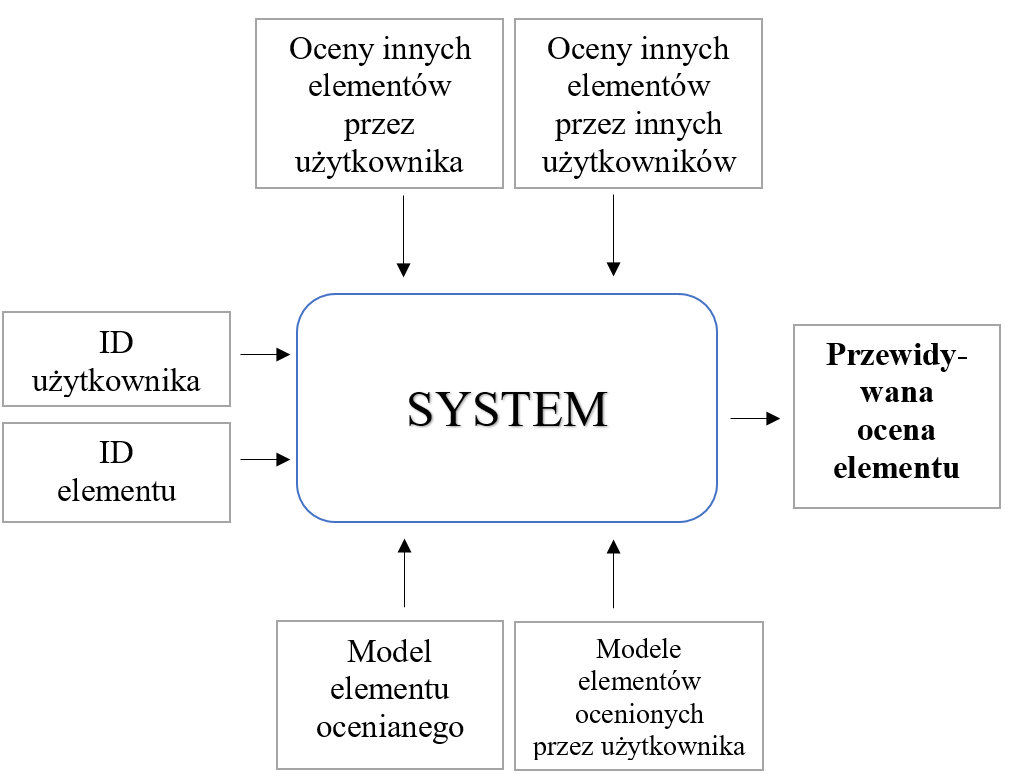
\includegraphics[width=0.7\textwidth]{blackbox}
   	\caption{Model czarnoskrzynkowy}
   	\label{fig:blackbox}
 \end{figure}
 
 Założeniem systemu jest uniwersalność, zatem model elementu jest uogólniony i dostosowuje się w zależności do domeny, w której system jest wykorzystywany. Rys. \ref{fig:modelElementu} przedstawia reprezentację elementu w systemie. W zbiorze wartości mogą znaleźć się takie pozycje jak lista aktorów, reżyser (w przypadku filmów), gatunek, wykonawca (w przypadku muzyki), typ produktu lub cena (w przypadku systemów typu e-commerce).
 
 \begin{figure}[!ht] 
 	\centering
 	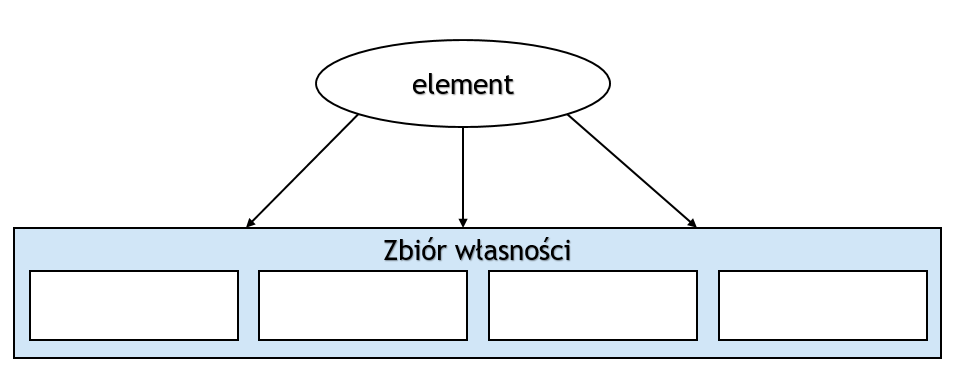
\includegraphics[width=0.7\textwidth]{modelElementu}
 	\caption{Uogólniony model elementu}
 	\label{fig:modelElementu}
 \end{figure}
 
 Każdy użytkownik systemu jest anonimowy. Nie jest znana jego płeć, wiek, pochodzenie itp. System nie przechowuje także informacji właściwych mediom społecznościowym, takich jak relacje między użytkownikami (przyjaźnie, śledzenie). Wiadomym jest jedynie, jakie elementy zostały ocenione i jak zostały ocenione. Rys. \ref{fig:modelUsera} przedstawia reprezentację użytkownika w systemie.
 
 \begin{figure}[!ht] 
  	\centering
  	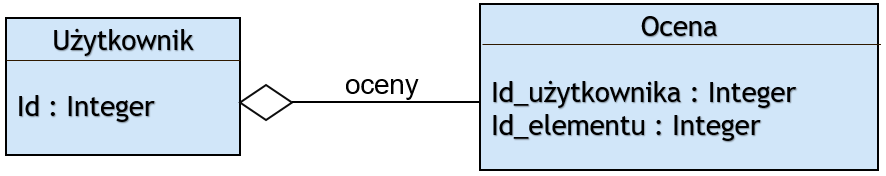
\includegraphics[width=0.7\textwidth]{modelUsera}
  	\caption{Uogólniony model elementu}
  	\label{fig:modelUsera}
  \end{figure}


 \chapter{Algorytmy}
 \shortTitle{Algorytmy}

	\todo{Napisać wstęp. Co powinien zawierać?}

	 \section{Filtrowanie kolaboratywne}
	 
		 Implementacja algorytmów collaborative--filtering, które wykorzystane zostały w projekcie pochodzą biblioteki MyMediaLite \cite{mymedialite,gantner2011mymedialite}. 
	 
		 Przed podjęciem decyzji dotyczącej wyboru algorytmu kolaboratywnego filtrowania zostały przeanalizowane testy na bazie MovieLens M1 \cite{harper2016movielens}. Testy przeprowadzone zostały z pięciokrotną walidacją krzyżową. Rys. \ref{fig:cfcomparision} przedstawia wyniki (im mniejsza wartość RMSE i MAE tym lepiej). 
	 
		 \begin{figure}[!ht] 
		 	\centering
		 	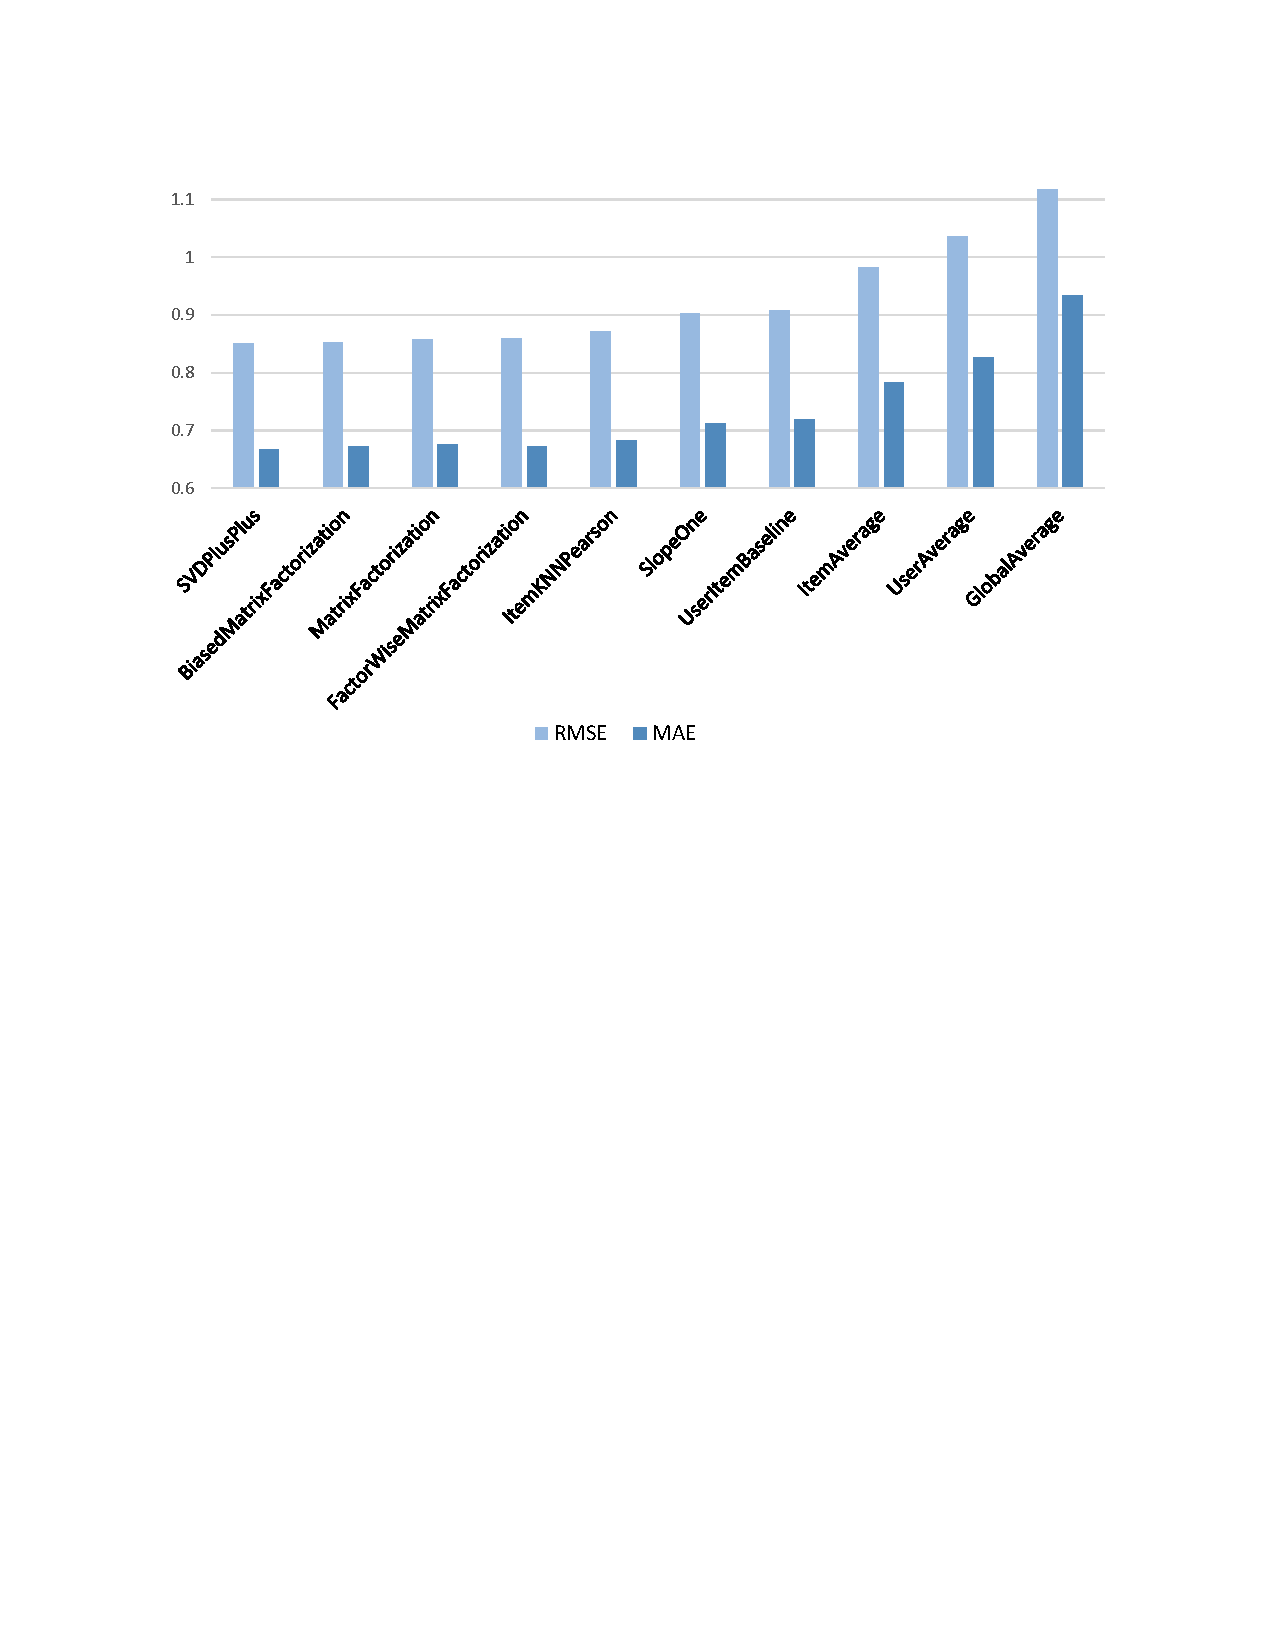
\includegraphics[width=1\textwidth]{cfcomparision}
		 	\caption{Test algorytmów filtrowania kolaboratywnego \protect\cite{mymedialitedatasets}}
		 	\label{fig:cfcomparision}
		 \end{figure}
	 
		 \todo{"chyba będzie lepiej jednak przenieść te algorytmy do rozdziału z przeglądem, bo tutaj raczej czytelnik oczekuje już konkretnego algorytmu" --- omówić reorganizację}
	 
		 Najefektywniejsze okazały się algorytmy SVD++, Biased Matrix Factorization i Matrix Factorization bazujące na podejściu model--based. 
	 	 
		 \subsection{Matrix Factorization}
		
		 \subsubsection{Metoda matematyczna}	
	
		 Algorytm \textit{Matrix Factorization} bazuje na matematycznej metodzie rozkładu macierzy na czynniki.
	
	
			  \begin{figure}[!ht] 
			  	\centering
			  	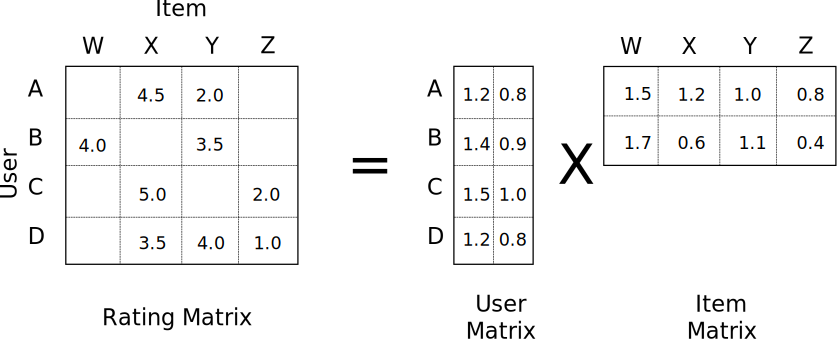
\includegraphics[width=1\textwidth]{factorization}
			  	\caption{Faktoryzacja macierzy \protect\cite{id:ComputingRecommendationsExtremeScaleApacheFlink}}
			  	\label{fig:factorization}
			  \end{figure}
			 
		Początkowo dana jest niekompletna macierz zawierająca oceny, jakie użytkownicy wystawili konkretnym elementom (\textit{Rating Matrix}). Celem metody jest odnalezienie wartości, jakie można wstawić w puste miejsca, czyli przewidzenie jaką ocenę dany użytkownik wystawi nieocenionemu jeszcze elementowi. 		
		
		W tym celu tworzone są odrębne macierze dla użytkowników i elementów zawierające ukryte własności. Każdy element powiązany jest z wektorem $q_i \in \mathbb{R} ^f$ (wektory W, X, Y, Z na rys. \ref{fig:factorization}) a każdy użytkownik z wektorem $p_u \in \mathbb{R} ^f$ (wektory A, B, C, D na rys. \ref{fig:factorization}). Wartości czynników ukrytych determinują stopień zainteresowania daną cechą (w przypadku macierzy użytkowników) bądź stopień, w jakim dany element posiada tę cechę (w przypadku macierzy elementów).		
		
		Iloczyn skalarny $q_i^T p_u$ przedstawia relację pomiędzy użytkownikiem a elementem. Na tej podstawie można wnioskować ocenę $r_{ui}$, jaką użytkownik może wystawić elementowi: $r_{ui} = q_i^T p_u$ i w konsekwencji estymować zainteresowanie użytkownika danym elementem \cite{koren2009matrix}.
		
		Głównym wyzwaniem jest odnalezienie wartości macierzy użytkownika i elementu, które po przemnożeniu przez siebie dadzą kompletną macierz ocen. W przypadku omawianych algorytmów stosowana jest metoda stochastycznego gradientu prostego. 
			
		\subsubsection{Stochastyczny gradient prosty}
			
		Stochastyczny gradient prosty (ang. \textit{stochastic gradient descent}, \textit{SGD}) jest iteracyjnym algorytmem optymalizacyjnym mającym za zadanie odnalezienie minimum bądź maksimum zadanej funkcji. Jest on uproszczeniem popularnej metody gradientu prostego \cite{bottou2012stochastic}.
				 
		Dana jest funkcja celu w postaci
		
		\begin{equation}
		\label{eq:sgd1}
		Q(w) = \sum_{i=1}^{n}Q_i(w)
		\,.
		\end{equation}
			
		Zadaniem algorytmu jest odnalezienie takiej wartości parametru $w$, dla którego $Q(w)$ będzie minimalne. Wykorzystując klasyczną metodę gradientu prostego poszukiwania można zapisać następującym wzorem:
		
		\begin{equation}
		\label{eq:sgd2}
		w:= w - \eta \sum_{i=1}^{n} \nabla Q_i(w)
		\,,
		\end{equation}
			
		gdzie $\eta$ symbolizuje współczynnik uczenia (ang. \textit{learning rate}). W przypadku algorytmu stochastycznego następuje uproszczenie. Zamiast obliczać dokładny gradient $Q(w)$, w każdej iteracji jest  on aproksymowany na podstawie pojedynczego, losowo wybranego przypadku:
		
		\begin{equation}
		\label{eq:sgd3}
		w:= w - \eta \nabla Q_i(w)
		\,.
		\end{equation}
			
		Algorytm przetwarza wszystkie elementy zbioru treningowego i dla każdego przypadku wykonuje aktualizację wartości $w$. Przebieg algorytmu przedstawiony jest poniżej (algorytm \ref{aq:sgd}).
			
		\def\alghoritm5{Stochastyczny gradient prosty}
		\begin{algorithm}[!ht]
			\caption{\alghoritm5}
			\myalgorithm{\alghoritm5}
			\label{aq:sgd}
			\begin{algorithmic}
				\STATE $w \leftarrow \text{początkowy wektor } w$
				\STATE $\eta \leftarrow \text{współczynnik uczenia}$
				
				\WHILE{nie odnaleziono minimum}
				
				\STATE losowo mieszkaj przykłady ze zbioru testowego
				\FOR {$i \in \{1, 2, \ldots, n\} $}
					\STATE $w:= w - \eta \nabla Q_i(w)$
				\ENDFOR
				\ENDWHILE
			\end{algorithmic}
		\end{algorithm}
			 
		Stochastyczny gradient prosty wykonuje dużo więcej kroków niż jego klasyczny odpowiednik aby odnaleźć rozwiązanie optymalne. Mimo tego jest on szybszy, gdyż każdy pojedynczy krok jest mniej kosztowny niż w oryginale. Różnicę w działaniu przedstawia rys. \ref{fig:sgd}.  
			 
		 \begin{figure}[!ht] 	
		 	\centering	 		 	
		 	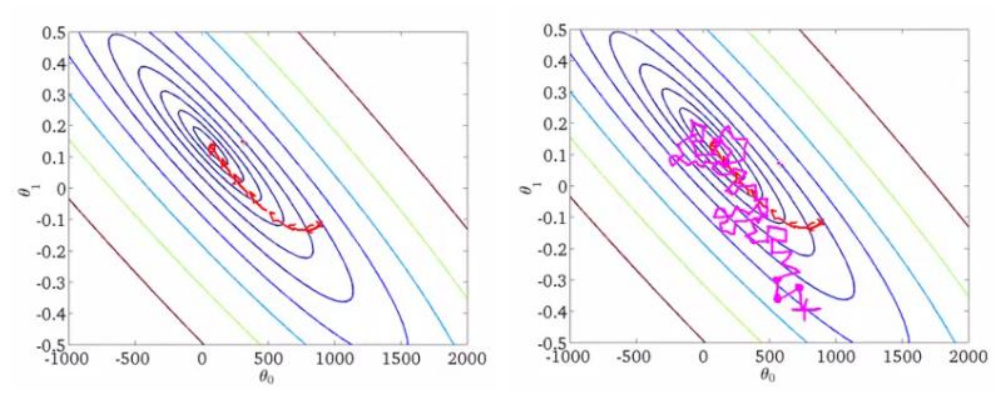
\includegraphics[width=0.5\textwidth]{sdg}
		 	\caption{Różnica pomiędzy klasycznym gradientem prostym (po lewej) a jego stochastyczną wersją (po prawej) \protect\cite{effandpractstochsub}}
		 	\label{fig:sgd}
		 \end{figure}
			 
		\newpage
		\subsubsection{Przebieg algorytmu Matrix Factorization}
			 
		Przebieg algorytmu składa się z dwóch faz. W pierwszej fazie inicjowany jest model (zob. algorytm \ref{aq:mf_init}). Daną wejściową jest macierz zawierająca dotychczasowe oceny  elementów przez użytkowników w systemie. Na wyjściu otrzymywane są dwie nowe macierze reprezentujące ukryte własności użytkowników i elementów. Na tym etapie \todo{OMÓWIĆ dwa ostatnie zdania brzmią razem tak, jakby wynik był losowy} są one wypełnione wartościami losowymi. 		

	
		\def\alghoritm1{Matrix Factorization -- Inicjacja modelu}
		\begin{algorithm}[H]
			\caption{\alghoritm1}
			\myalgorithm{\alghoritm1}
			\label{aq:mf_init}
			\begin{algorithmic}
				\STATE $N \leftarrow \text{liczba użytkowników}$
				\STATE $M \leftarrow \text{liczba elementów}$
				\STATE $F \leftarrow \text{liczba ukrytych własności}$
				\STATE $ratings \leftarrow \text{Macierz NxM zawierająca dotychczasowe oceny wszystkich elementów }$
				\STATE $\text{przez wszystkich użytkowników}$
				\STATE $user\_factors \leftarrow \text{Macierz NxF reprezentująca ukryte własności użytkowników}$
				\STATE $item\_factors \leftarrow \text{Macierz MxF reprezentująca ukryte własności elementów}$
				
				\FOR{each $uf \in user\_factors$, $if \in item\_factors$ }
				\STATE wstaw losową wartość za pomocą transformacji Boxa--Mullera
				\ENDFOR

				\FOR{each $user, item \in ratings$ }			
					\IF {$ratings_{user,item} = NULL$}
					\STATE wstaw 0 do wiersza $user\_factors_{user}$ i $item\_factors_{item}$
					\ENDIF				
				\ENDFOR
				\RETURN $user\_factors, item\_factors$
			\end{algorithmic}
		\end{algorithm}
	
		
		W fazie drugiej następuje uczenie metodą stochastycznego gradientu prostego (zob. algorytm  \ref{aq:mf_learn}). Wynikiem tej fazy są macierze reprezentujące ukryte własności użytkowników i elementów. Mnożąc je ze sobą uzyskiwana jest przewidywana ocena każdego z elementów przez użytkowników. 
		
		Przed rozpoczęciem uczenia ustalane są parametry: parametr regulujący (ang. \textit{regularization}), współczynnik uczenia (ang. \textit{learning rate}), parametr zanikania (ang. \textit{decay}) i liczba iteracji. 	
		W trakcie trwania głównej pętli parametr regulujący pozostaje niezmienny. Służy on zapobieganiu zjawisku nadmiernego dopasowania (ang. \textit{overfitting}). Tempo uczenia jest przy każdym przebiegu pętli mnożone przez parametr zanikania, dzięki czemu można kontrolować w jakim stopniu kolejne przebiegi pętli wpływają na finalny wynik. 
		
		Ostatnim parametrem ustalanym przed główną pętlą jest skośność globalna (ang. \textit{global bias}), która jest średnią wszystkich znanych ocen. 
		
		W pętli uczenia wykonywane są następujące operacje: dla każdej pary użytkownik -- element budowana jest przewidywana ocena poprzez obliczenie iloczynu skalarnego odpowiednich wartości z macierzy wartości ukrytych. Ocena ta jest modyfikowana poprzez dodanie globalnej skośności a następnie porównywana z faktyczną oceną elementu przez użytkownika. Tak uzyskany błąd służy do wyliczenia delty. Macierze wartości ukrytych uaktualniane są o wyliczoną deltę. 
		
		Pod koniec każdej iteracji aktualizowany jest współczynnik uczenia.
	
		\def\alghoritm2{Matrix Factorization -- Faza uczenia}
		\begin{algorithm}[H]
			\caption{\alghoritm2}
			\myalgorithm{\alghoritm2}
			\label{aq:mf_learn}
			\begin{algorithmic}
				\STATE $global\_bias \leftarrow \text{średnia wszystkich ocen}$
				\STATE $X \leftarrow \text{liczba iteracji}$			
				\STATE $regularization \leftarrow \text{parametr regulujący}$			
				\STATE $current\_learnrate \leftarrow \text{współczynnik uczenia}$
				\STATE $decay \leftarrow \text{paramert zanikania}$
				
				\FOR{each $x \in X$ }
					\FOR{each $user, item \in ratings$ }
					
						\STATE $predicion= global\_bias + IloczynSkalarny(user\_factors_{user}, item\_factors_{item}); $
					
						\STATE $error = ratings_{user,item} - prediction$
				
						\textbf{//dopasowanie własności ukrytych:}
				
						\FOR{each $f \in F$}
							\STATE $delta_u = error * item\_factors_{item, f} - regularization * user\_factors_{user, f}$
							\STATE $delta_i = error * user\_factors_{user, f} - regularization * item\_factors_{item, f}$
							
							\STATE $user\_factors_{user, f} \incr current\_learnrate * delta_u$
							\STATE $item\_factors_{item, f} \incr current\_learnrate * delta_i$
						\ENDFOR					
					\ENDFOR			
					\STATE $current\_learnrate \incrtimes decay$				
				\ENDFOR
				\RETURN $user\_factors, item\_factors$
			\end{algorithmic}
		\end{algorithm}
	
	
		 \subsection{Biased Matrix Factorization}
		 
		 Algorytm \textit{Biased Matrix Factorization} jest modyfikacją wyżej opisanego algorytmu \textit{Matrix Factorization}. Podobnie jak jego pierwowzór składa się z dwóch faz. W pierwszej fazie dodatkowo inicjowane są dwa dodatkowe wektory: skośność użytkowników (ang. \textit{user bias}) i skośność elementów (ang. \textit{item bias}). 
		 
		 Inaczej jest też obliczana skośność globalna: 
 		 
		 \begin{equation}
		 \label{eq:global_bias}
		 global\_bias = 
		 \frac
		 { 
		 	\frac{ a - r_{min} }{ r_{max} - r_{min} }
		 }
		 {
		 	1 - \frac{ a - r_{min} }{ r_{max} - r_{min} }	
		 }
		 \,,
		 \end{equation} 
		 		
		 gdzie
		 
		 \begin{conditions*}
		 	a & to średnia wszystkich ocen \\
		 	r_{min}  &  to minimalna ocena w systemie  \\
		 	r_{max}  &  to maksymalna ocena w systemie
 		 \end{conditions*} 
		 
		 Faza druga wygląda podobnie jak w przypadku algorytmu \textit{Matrix Factorization}, jednak są uwzględniane dodatkowe parametry i wykonywane dodatkowe kroki.
		 
		 \def\alghoritm3{Biased Matrix Factorization -- Faza uczenia}
		 \begin{algorithm}[H]
		 	\caption{\alghoritm3}
		 	\myalgorithm{\alghoritm3}
		 	\label{aq:bmf_learn}
		 	\begin{algorithmic}
		 		\STATE $global\_bias \leftarrow \text{średnia wszystkich ocen}$
		 		\STATE $X \leftarrow \text{liczba iteracji}$			
		 		\STATE $regU, regI, BiasReg \leftarrow \text{parametry regulujące dla użytkownika, elementu i ogólny }$			
		 		\STATE $current\_learnrate \leftarrow \text{współczynnik uczenia}$
				\STATE $BiasLearnRate \leftarrow \text{współczynnik uczenia skośności}$
		 		\STATE $decay \leftarrow \text{paramert zanikania}$
		 		
		 		\FOR{each $x \in X$ }
			 		\FOR{each $user, item \in ratings$ }			 		
				 		\STATE $score= global\_bias + user\_bias_{user} + item\_bias_{item} + IloczynSkalarny(user\_factors_{user}, item\_factors_{item})$
				 		
				 		\STATE $sig\_score = \frac{1}{1 + \exp(-score)}$
				 		
				 		\STATE $predicion= rating_{min} + sig\_score + (rating_{max} - rating_{min}) $
				 		
				 		\STATE $error = ratings_{user,item} - prediction$
				 		
				 		\STATE $gradient\_common = err * sig\_score * (1 - sig\_score) * (rating_{max} - rating_{min})$
				 		
				 		\textbf{//dopasowanie skośności:}
				 		
				 		\STATE $user\_bias_{user} \incr BiasLearnRate * current\_learnrate * (gradient\_common - BiasReg * RegU * user\_bias_{user})$
				 		
				 		\STATE $item\_bias_{item} \incr BiasLearnRate * current\_learnrate * (gradient\_common - BiasReg * RegI * item\_bias_{item})$
				 		
				 		\textbf{//dopasowanie własności ukrytych:}
				 		
				 		\FOR{each $f \in F$}
					 		\STATE $delta_u = gradient\_common * item\_factors_{item, f} - RegU * user\_factors_{user, f}$
					 		
					 		\STATE $delta_i = gradient\_common * user\_factors_{user, f} - RegI * item\_factors_{item, f}$
					 		
					 		\STATE $user\_factors_{user, f} \incr current\_learnrate * delta_u$
					 		\STATE $item\_factors_{item, f} \incr current\_learnrate * delta_i$
				 		\ENDFOR					
			 		\ENDFOR			
			 		\STATE $current\_learnrate \incrtimes decay$				
		 		\ENDFOR
		 		\RETURN $user\_factors, item\_factors$
		 	\end{algorithmic}
		 \end{algorithm}
		 		 
		 \subsection{SVD++}
		 
		 SVD++ jest rozszerzeniem metody SVD (dekompozycja głównych składowych, ang. \textit{singular value decomposition}). Od poprzednich omawianych algorytmów różni go przede wszystkim to, że korzysta nie tylko z podejścia aktywnego do tworzenia profilu użytkownika ale także z pasywnego (zob. \ref{ss:metody_tworzenia_profilu_uzytkownika}).
		 
		 Model SVD++ opisywany jest równaniem:
		 
		 \begin{equation}
		 	\label{eq:svd}
		 	r_{ui} = \mu + b_u + b_i + q_i^T (p_u + \frac{1}{\sqrt{|N(u)|}} \sum_{j \in N(u)}^{} y_j) 
		 	\,,
		 \end{equation}
		 		 
		 Użytkownik powiązany jest z wektorem $p_u \in \mathbb{R} ^f$ reprezentującym zainteresowanie konkretnymi cechami. Taki model uzupełniany jest sumą  $\frac{1}{\sqrt{|N(u)|}} \sum_{j \in N(u)}^{} y_j$, która reprezentuje informacje niejawne (\textit{implicit feedback}). Przykładem informacji niejawnej jest fakt, że użytkownik w ogóle zareagował na dany element (np. ocenił go), bez względu na wynik tej interakcji. 
		  
		 Zmienne $b_u$ i $b_i$ reprezentują obserwowane odchylenie od średniej dla użytkowników i elementów, natomiast $\mu$ to średnia wszystkich ocen \cite{koren2008factorization}. 
		 	 
		 
	 \section{Filtrowanie z analizą zawartości}
	 
		 Algorytmy content-based budują rekomendację na podstawie ocen, jakie zostały dotychczas wystawione przez użytkownika. Analizowane są cechy elementów i ich wartości oraz określana jest ich siła wpływu na finalną ocenę. 
		 
		 W tym celu dla każdego użytkownika tworzona jest sieć neuronowa, która uczy się jego preferencji. 
		 
		 W projekcie wykorzystana została implementacja sieci neuronowych z biblioteki AForge.NET Framework \cite{aforgenet}.
	 
		 \subsection{Konstrukcja sieci neuronowej}
		 
		 \subsubsection{Struktura perceptronów}
		 \label{sss:strukturaperceptronow}
		 
		 Sieć neuronowa składa się z trzech warstw neuronów (perceptronów). W każdej warstwie wszystkie neurony mają konstrukcję na jak rys. \ref{fig:schematneuronu}
		 
 		 \begin{figure}[!ht] 		 		 	
	 		 	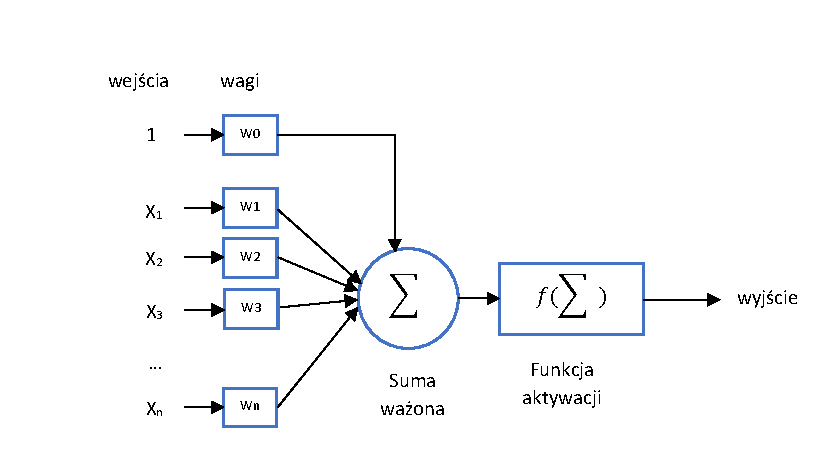
\includegraphics[width=0.9\textwidth]{schematneuron}
	 		 	\caption{Schemat perceptronu}
	 		 	\label{fig:schematneuronu}
 		 \end{figure}
		 
		 Do neuronu przekazywany jest zestaw wartości w postaci wektora $x$. Następnie obliczana jest suma ważona tych wartości w zależności od nadanych wag $w$. Proces dobierania odpowiednich wag jest nazywany uczeniem (zob. \ref{ss:uczeniesiecineuronowej}). W następnym kroku suma ważona przekazywana jest do funkcji aktywacji neuronu. Jeżeli funkcja przyjmie wartość wyższą lub równą niż określony próg aktywacji, to perceptron zostanie pobudzony (zwróci wartość 1). Proces ten obrazuje równanie \ref{eq:neuroneq}.
		 
		 \begin{equation}
		 \label{eq:neuroneq}
		 N(x_1, x_2, x_3, \ldots, x_n) = 
			 \begin{cases}
			 1       & \quad \text{jeśli } f(w_0 + \sum_{i=1}^{n}w_ix_i) \geq \eta\\
			 0		 & \quad \text{jeśli } f(w_0 + \sum_{i=1}^{n}w_ix_i) < \eta\\
			 \end{cases}
		 \,,
		 \end{equation}
		 
		 gdzie
		 
		 \begin{conditions*}
		 	w & to wagi kolejnych wejść \\
		 	x & to wartości przekazywane do wejść \\
		 	f(u) & to funkcja aktywacji neuronu \\
		 	\eta & to próg aktywacji neuronu
		 \end{conditions*} 
		 
		 Na potrzeby algorytmu rekomendacji zdecydowano się przyjąć sigmoidalną unipolarną funkcję aktywacji neuronu (równanie \ref{eq:sigmoidal}). Funkcja przyjmuje wartości z zakresu $[0,1]$.
		 
		  \begin{equation}
		  \label{eq:sigmoidal}
		  f(x) = \frac{1}{1 + \exp(-\alpha x)}
		  \,.
		  \end{equation}

		 Wykres funkcji wygląda jak na rys. \ref{fig:sigmoid}.

 		 \begin{figure}[!ht] 
			\centering
			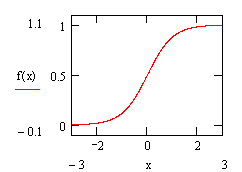
\includegraphics{sigmoid}
			\caption{Wykres sigmoidalnej funkcji aktywacji perceptronu \protect\cite{aforgenet}}
			\label{fig:sigmoid}
		 \end{figure}

		 \subsubsection{Struktura sieci i przebieg algorytmu}
		 
		 Pierwszym etapem algorytmu jest analiza cech elementów ocenionych przez użytkownika. Tworzona jest lista wszystkich występujących cech które powtarzają się minimum tyle razy, ile wynosi wartość  parametru \textit{minimumRepeatingFeatures}. 
		 
		 Następnie inicjowana jest sieć neuronowa. Ilość neuronów warstwy wejściowej jest równa ilości wyodrębnionych cech. Warstwa ukryta zawiera tyle neuronów ile jest to określone parametrem \textit{hiddenLayerNeurons}. Warstwa wyjściowa składa się z tylko jednego neuronu (rys. \ref{fig:siecneuronowa}). 
		 
		 \begin{figure}%[H] %!ht 
		 	\centering
		 	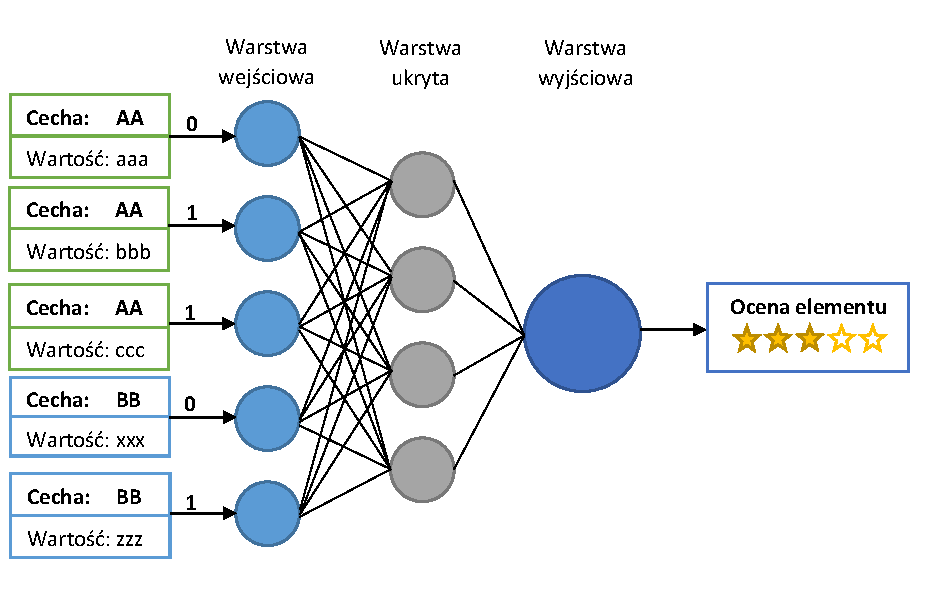
\includegraphics[width=1\textwidth]{siecneuronowa}
		 	\caption{Schemat sieci neuronowej}
		 	\label{fig:siecneuronowa}
		 \end{figure}
		 
		 W kolejnym etapie dla każdego elementu tworzona jest mapa cech. Jeżeli element zawiera daną cechę o danej wartości przypisywana jest wartość $1$. W przeciwnym razie wstawiane jest $0$. Rys. \ref{fig:mapacech} przedstawia przykładową mapę cech. Tak przygotowana lista przekazywana jest do sieci neuronowej. 
		 
		 \begin{figure}%[H]  %!ht
		 	\centering
		 	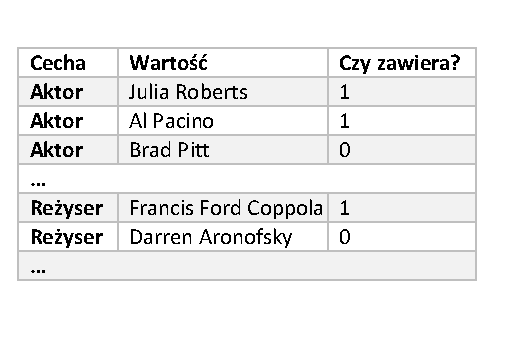
\includegraphics[width=0.7\textwidth]{mapacech}
		 	\caption{Mapa cech elementu. Wiadomo, że element X zawiera cechę ,,Aktor'' o wartościach ,,Julia Roberts, Al Pacino'' oraz cechę ,,Reżyser'' o wartości ,,Francis Ford Coppola''. Element nie zawiera cechy ,,Aktor'' o wartości ,,Brad Pitt'' ani cechy ,,Reżyser'' o wartości ,,Darren Aronofsky'' więc w te miejsca wstawiane jest $0$.}
		 	\label{fig:mapacech}
		 \end{figure}
		 
		 Na wyjściu sieć zwraca przewidywaną ocenę elementu.
		 		 
		 
		 \subsection{Uczenie sieci neuronowej}
		 \label{ss:uczeniesiecineuronowej}
		 
		 Aby sieć zwracała jak najlepsze wyniki musi wcześniej zostać nauczona preferencji użytkownika. Uczenie sieci polega na odnalezieniu odpowiednich wag dla każdego wejścia każdego perceptronu sieci (budowa perceptronu zob. \ref{sss:strukturaperceptronow}). Proces ten można zapisać w postaci
		 
		 \begin{equation}
		 \label{eq:weightadaptation}
		 W_{ij}(n+1) = W_{ij}(n) + \Delta W_{ij}(n) 
		 \,,
		 \end{equation}
		 		 
		 gdzie
		 
		 \begin{conditions*}
		 	W_{ij}(n) & to poprzednie wagi wejść \\
		 	W_{ij}(n+1) & to nowe wagi wejść \\
		 	n & numer cyklu uczącego 
		 \end{conditions*} 
		 
		 Dostrajanie wartości wag można wykonać na wiele sposobów. Można wyróżnić uczenie nadzorowane (z nauczycielem), uczenie z krytykiem (ang. \textit{reinforcement learning}) i uczenie samoorganizujące się (bez nadzoru) \cite{osowski1996sieci}.
		 
		 Na potrzeby systemu rekomendacji content-based opisywanego w tej pracy wykorzystane zostały trzy metody uczenia: algorytm propagacji wstecznej, algorytm RPROP i algorytm genetyczny. Wymienione metody należą do kategorii uczenia nadzorowanego. 
		 
		 
		 \subsection{Propagacja wsteczna}
	 
		 Algorytm propagacji wstecznej jest jedną z popularniejszych metod uczenia nadzorowanego jednokierunkowych sieci neuronowych. Zbiór uczący składa się z danych wejściowych (wektory cech elementu) i z informacji o oczekiwanym wyniku (ocena elementu). Różnica między wynikiem zwróconym przez sieć a wartością oczekiwaną stanowi miarę błędu sieci neuronowej. 
		 
		 \begin{figure}[!ht] 
	 		 	\centering
	 		 	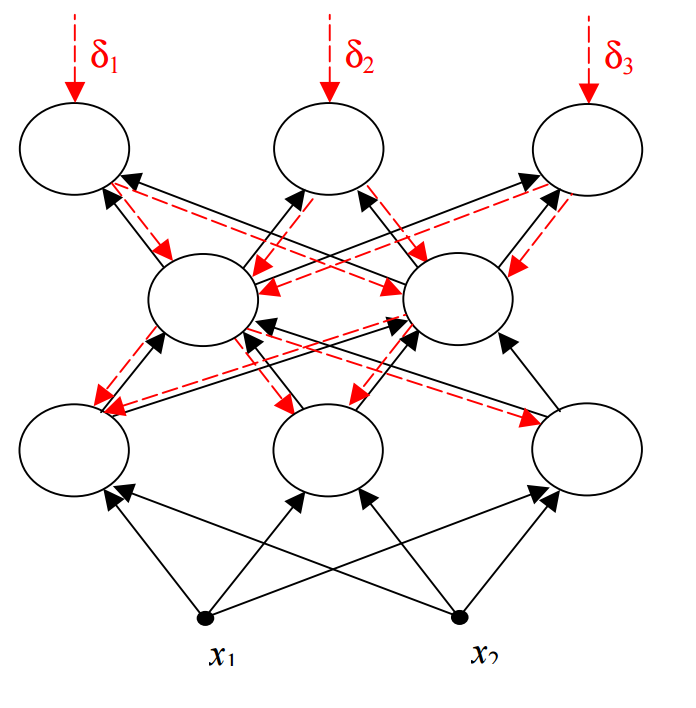
\includegraphics[width=0.5\textwidth]{ilustracjabackprop}
	 		 	\caption{Algorytm propagacji wstecznej w sieci trójwarstwowej -- idea działania \protect\cite{kwateralgorytmy}}
	 		 	\label{fig:ilustracjabackprop}
		 \end{figure}
		 
		 Wiadomo, że funkcja celu jest funkcją ciągłą. Bazując na gradientowych metodach optymalizacji, wagi w sieci neuronowej aktualizowane są w następujący sposób:	 
		 
 		 \begin{equation}
 		 \label{eq:weightadaptation3}
 		 W_{ij}(n+1) = W_{ij}(n) + \Delta W_{ij}(n) 
 		 \,,
 		 \end{equation}
 		 
 		 
 		 \begin{equation}
 		 \label{eq:weightadaptation2}
 		 \Delta W_{ij}(n) = \eta p(W)
 		 \,,
 		 \end{equation}
		 
		 gdzie
		 
		 \begin{conditions*}
		 	\eta & to współczynnik uczenia (ang. \textit{learning rate}) \\
		 	p(W) & to kierunek w przestrzeni wielowymiarowej W 
		 \end{conditions*} 
		 
		 Aby wyznaczyć kierunek $p(W))$ dla wszystkich warstw sieci należy przejść przez kolejne etapy uczenia \cite{haykin1994neural,hertz1993wstkep,kwateralgorytmy,osowski1996sieci,timothy1996sieci}.
		 
		 \begin{enumerate}
		 	\item W kroku pierwszym sieć neuronowa poddawana jest analizie o zwykłym kierunku przepływu sygnałów. Wynikiem są wartości sygnałów wychodzących z neuronów warstw wyjściowej i ukrytych oraz pochodne funkcji aktywacji w kolejnych warstwach. 
		 	
		 	\item W kroku drugim kierunek przepływu sygnałów zostaje odwrócony (stąd nazwa propagacja wsteczna). Funkcje aktywacji zostają zastąpione przez swoje pochodne. Na oryginalne wyjście sieci (aktualnie wejście) podana zostaje wartość równa różnicy pomiędzy wynikiem oczekiwanym a wynikiem zwróconym przez sieć. 
		 	
		 	\item Obliczana zostaje wartość różnic wstecznych.
		 	
			\item W kolejnym kroku następuje wreszcie proces adaptacji wag. Odbywa się on zarówno dla sieci zwykłej jak i dla sieci o propagacji wstecznej. Reguła modyfikacji ma postać: 

			\begin{equation}
				\label{eq:weightadaptation4}
				\Delta W_{ij} = \eta \sum_\text{wzroce}^{} \delta_\text{wyjście} \cdot x_\text{wejście}
				\,,
			\end{equation}
			
			\item Powyższe kroki potarzane są dla każdej pary dane wejściowe -- oczekiwany wynik tak długo, aż poziom błędu spadnie poniżej akceptowalnej wartości bądź osiągnięta zostanie maksymalna liczba iteracji. 

		 \end{enumerate}
				 
		 Algorytm propagacji wstecznej obrazuje schemat blokowy \ref{fig:propagacjawsteczna}.
		 
			\begin{figure}[!ht] 
				\centering
				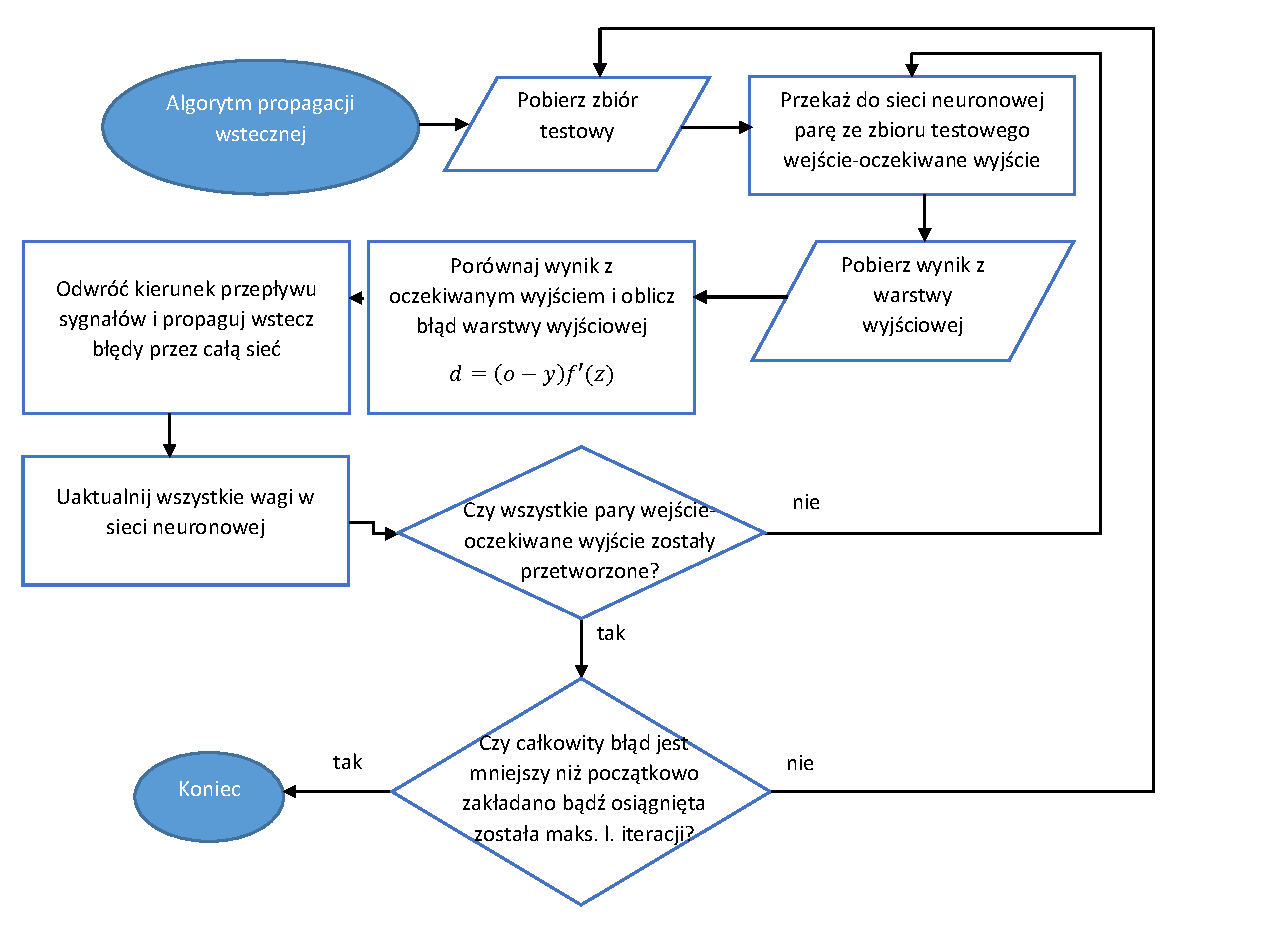
\includegraphics[width=1\textwidth]{propagacjawsteczna}
				\caption{Algorytm propagacji wstecznej}
				\label{fig:propagacjawsteczna}
			\end{figure}
			
		 \subsubsection{Metoda momentum}
		 \label{sss:metoda_momentum}
	 
		 W celu zwiększenia efektywności działania algorytmu została zastosowana metoda momentum. I tak też standardowy sposób aktualizacji wag sieci (równanie \ref{eq:weightadaptation3}) został zmodyfikowany w następujący sposób:
		 
		 \begin{equation}
		 \label{eq:zasadamomentum1}
		 W_{ij}(n+1) = W_{ij}(n) + \Delta W_{ij}(n) 
		 \,,
		 \end{equation}
		 
		 \begin{equation}
		 \label{eq:zasadamomentum2}
		 \Delta W_{ij}(n) = \eta(n) \cdot p(n) + \alpha(W_{ij}(n)-W_{ij}(n-1)) 
		 \,,
		 \end{equation}
		 
		 gdzie $\alpha$ jest współczynnikiem momentum z zakresu $[0,1]$. Im wyższa wartość współczynnika tym większy jego wpływ na ostateczny kształt kolejnych wag. W dalszej części pracy przeprowadzono eksperymenty mające na celu dobranie optymalnej wartości współczynnika momentum.
		 
 		 \subsection{Algorytm RPROP}		 
		 
		 Pomimo dużej popularności algorytmu propagacji wstecznej nie jest on pozbawiony wad. Sporym problemem jest jego relatywnie niska szybkość działania, szczególnie w przypadku bardzo dużych sieci neuronowych -- a więc w przypadku odpowiadającemu potrzebom systemów rekomendacji. W odpowiedzi na te problemy Martin Riedmiller i Heinrich Braun zaproponowali w 1992 roku alternatywny algorytm -- Resilient Backpropagation (RPROP).
		 
		 Główną różnicą jest wykorzystywanie jedynie informacji o dodatniości lub ujemności każdej składowej gradientu zamiast o ich wartości (jak to się odbywa w oryginalnym algorytmie). Ponadto, współczynnik uczenia modyfikowany jest w każdym kolejnym kroku. 
		 
		 Modyfikacja współczynników odbywa się zgodnie ze wzorem:
		 
		 \begin{equation}
		 \label{eq:rprop}		 
		 \eta(t) = 
		 \begin{cases}
			min\{a \eta(t-1), \eta_{max}\}, & \quad \text{gdy } \frac{\partial E^2(t)}{\partial v(t)} \frac{\partial E^2(t-1)}{\partial v(t-1)} > 0 \\
			max\{b \eta(t-1), \eta_{min}\}, & \quad \text{gdy } \frac{\partial E^2(t)}{\partial v(t)} \frac{\partial E^2(t-1)}{\partial v(t-1)} < 0 \\
			\eta(n-1), & \quad \text{w każdym innym przypadku} 
		 \end{cases}		 
		 \,,
		 \end{equation}
		 
		 gdzie $\frac{\partial E^2(t)}{\partial v(t)}$ jest dokładną wartością składowej $v$ gradientu. Ponadto stałe $a$, $b$, $\eta_{min}$ i $\eta_{max}$ są zdefiniowane następująco:

		 \begin{conditions*}
		 	a = 1.2 \\
		 	b = 0.5 \\
		 	\eta_{min} = 10^{-6} \\
		 	\eta_{max} = 50
		 \end{conditions*} 
		 
		 Algorytm RPROP jest efektywniejszy pod kątem prędkości działania względem tradycyjnej propagacji wstecznej, więc dobrze sprawdza się tam, gdzie szybkość jest ważniejsza od wysokiej poprawności wyników \cite{riedmiller1993direct,riedmiller1994rprop}.
		 		 
 		 \subsection{Algorytm genetyczny}	
		 \label{ss:algorytm_genetyczny}
		 
		 Koncepcja algorytmów genetycznych została zaproponowana już 1960 roku przez Johna Hollanda. Należą one do klasy algorytmów ewolucyjnych, inspirowanych zasadą doboru naturalnego Darwina. Analogią do środowiska naturalnego jest pewien problem, dla którego poszukiwane jest optymalne rozwiązanie. Populacja składa się z potencjalnych rozwiązań, które są oceniane funkcją przystosowania. Zgodnie z zasadą Darwina zwycięża najsilniejszy, czyli najlepsze (chociaż nie zawsze optymalne) rozwiązanie \cite{pena2000evolutionary}. Schemat działania algorytmów genetycznych przedstawia rys. \ref{fig:algorytmgenetyczny}.	 
		 
		 
		 \begin{figure}[!ht] 
		 	\centering
		 	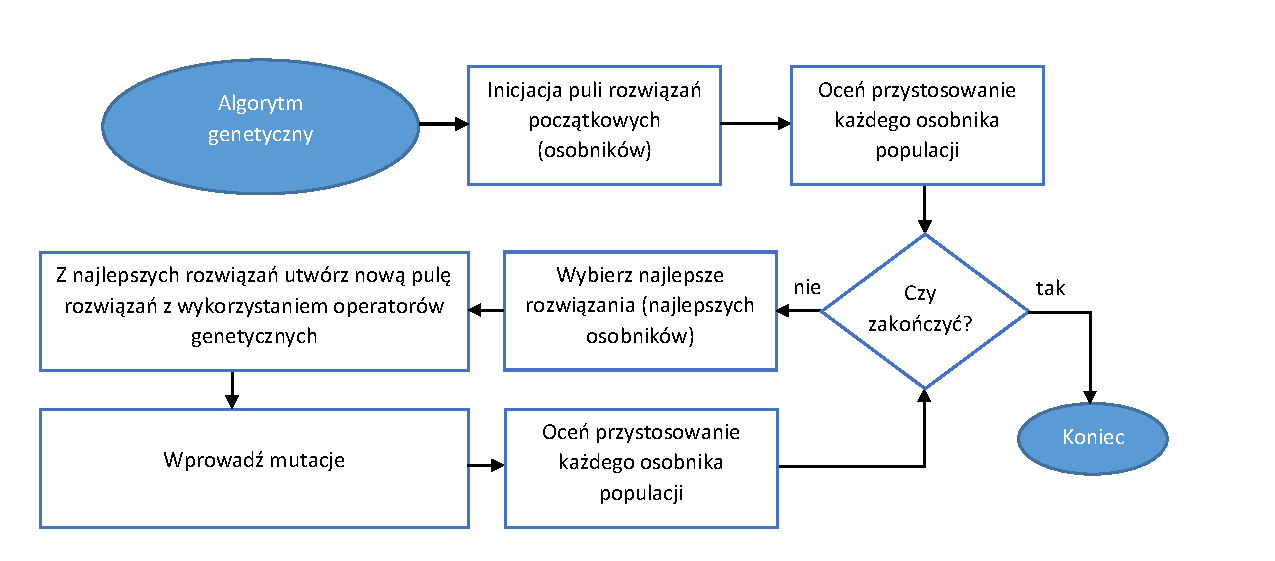
\includegraphics[width=1\textwidth]{algorytmgenetyczny}
		 	\caption{Ogólny schemat algorytmu genetycznego}
		 	\label{fig:algorytmgenetyczny}
		 \end{figure}

		 Jako, że algorytmy genetyczne należą do grupy algorytmów optymalizacyjnych mogą zostać wykorzystane do uczenia sieci neuronowych. W przypadku tej implementacji populację stanowią propozycje wag dla każdego perceptronu. Preferowane są takie zestawy wag, dla których sieć zwraca rezultaty obarczone najmniejszym błędem. Najlepsze zestawy są ze sobą krzyżowane oraz podlegają mutacji. W wyniku takich mechanizmów ewolucyjnych powstaje rozwiązanie, dla których sieć neuronowa zwraca oczekiwane rezultaty \cite{aforgenetgenetic,montana1989training}.
		 
		 
	 \section{Algorytymy hybrydowe}
		 
		 Zaproponowany nowy algorytm jest hybrydą metod collaborative i content-based. Zaimplementowanych zostało 9 wariantów:
		 
		 \begin{enumerate}
		 	\item Matrix Factorization + sieć neuronowa uczona metodą propagacji wstecznej;
		 	\item Matrix Factorization + sieć neuronowa uczona metodą RPROP;
		 	\item Matrix Factorization + sieć neuronowa uczona algorytmem genetycznym;
		 	\item Biased Matrix Factorization + sieć neuronowa uczona metodą propagacji wstecznej;
		 	\item Biased Matrix Factorization + sieć neuronowa uczona metodą RPROP;
		 	\item Biased Matrix Factorization + sieć neuronowa uczona algorytmem genetycznym;		 	
		 	\item SVD++ + sieć neuronowa uczona metodą propagacji wstecznej;
		 	\item SVD++ + sieć neuronowa uczona metodą RPROP;
		 	\item SVD++ + sieć neuronowa uczona algorytmem genetycznym.
		 \end{enumerate}
		 
		 Algorytm hybrydowy uruchamia osobno metodę filtrowania kolaboratywnego i filtrowania z analizą zawartości. W efekcie dla każdej pary użytkownik--element uzyskiwane są dwie  predykowane oceny z obu metod:  $r_{content-based_{ui}}$ i $r_{collaborative_{ui}}$. Ponadto, znany jest błąd $e$, z jakim zakończyło się uczenie sieci neuronowej dla użytkownika $u$. Przewidywana ocena obliczana jest wzorem:
		 
		 \begin{equation}
		 	\label{eq:hybrid}		 	
		 	 r_{ui} = (\frac{1}{k})^e \cdot r_{content-based_{ui}} + (1-(\frac{1}{k})^e) \cdot r_{collaborative_{ui}}
		 	\,,
		 \end{equation}
		 
		 gdzie $k$ jest parametrem konfigurowalnym (domyślnie $k = 2$), który determinuje stopień nachylenia funkcji wykładniczej. Parametr musi spełniać warunek $k>1$. Im wyższa wartość $k$, tym większy wpływ na rezultat ma wynik algorytmu kolaboratywnego. Zależność tę obrazuje rys. \ref{fig:hybridfunction}.
		 
		 \begin{figure}[!ht] 
		 	\centering
		 	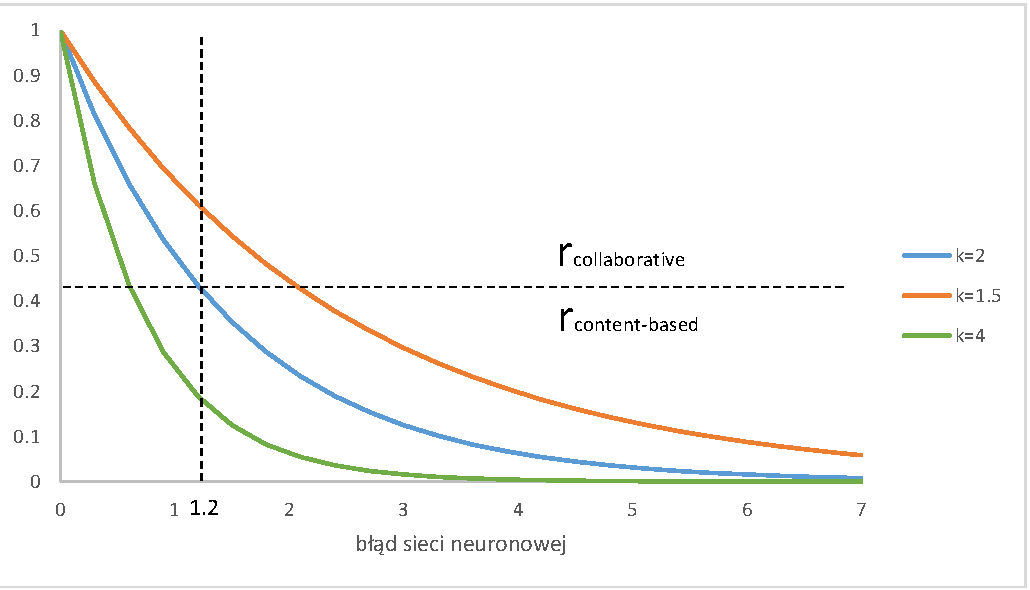
\includegraphics[width=0.7\textwidth]{hybridfunction}
		 	\caption{Wpływ parametru $k$ na wynik algorytmu}
		 	\label{fig:hybridfunction}
		 \end{figure}
	 
		 \subsection{Zalety zaproponowanej metody}
		 
		 Największą przewagą zaproponowanego algorytmu jest to, że łączy on zalety filtrowania z analizą zawartości i filtrowania kolaboratywnego minimalizując jednocześnie ich wady poprzez dynamiczne dobieranie proporcji ich wpływu na końcowy wynik. Nowa metoda cechuje się uniwersalnością, gdyż model elementu zawierający jego własności budowany jest automatycznie. Jednocześnie nie są wymagane informacje o użytkowniku inne, niż to jakie elementy ocenił i jak je ocenił. 
		 
		 Im więcej zostanie dostarczonych informacji na temat elementów, tym lepsze będą wyniki. Jednakże w przypadku braku takowych informacji metoda ciągle będzie działać,  wówczas wynik będzie opierał się głównie na rezultatach filtrowania kolaboratywnego.
		 
		 Analogicznie, w przypadku małej liczby powiązań z innymi użytkownikami, zaproponowany algorytm hybrydowy ulepszy wynik collaborative filtering dzięki czynnikowi content-based. 
		 
		 \subsection{Wady zaproponowanej metody}
		 
		 Największą wadą nowej metody jest wyższa złożoność. Czas budowania modelu jest sumą czasów budowania modeli kolaboratywnego i content-based. 
		 
		 Istnieje też ryzyko, że w momencie gdy wynik z metody collaborative będzie bardzo zły, to rezultat osiągnięty przez nową metodę będzie gorszy niż z samego filtrowania z analizą zawartości. 
	 
	 \section{Analiza złożoności i poprawności}
 
		 \todo{Analiza złożoności i poprawności}
 
\chapter{Ocena eksperymentalna}
\shortTitle{Ocena eksperymentalna}
	\section{Opis metody badawczej}
	
		\subsection{Miara oceny}
	
		W celu zbadania jakości algorytmów zostały zastosowane miary oceny: średnia kwadratowa błędów (RMSE) i średni błąd bezwzględny (MAE).
		
		\subsubsection{Średnia kwadratowa błędów}
	
		Średnia kwadratowa błędów (ang. RMSE -- \textit{root mean square error}) jest często wykorzystywaną miarą służącą zmierzeniu różnicy pomiędzy wartościami przewidywanymi a rzeczywistymi (obserwowanymi). 
		
		RMSE jest stosunkowo dobrą miarą dokładności ale tylko w celu porównania  różnych modeli dla tego samego zestawu danych. RMSE jest zależne od skali, zatem nie sprawdza się najlepiej w przypadku porównywania ze sobą różnych zmiennych \cite{hyndman2006another}.
		
		Średnią kwadratową błędów wylicza się ze wzoru:
		
		\begin{equation}
			\label{eq:rmse}
			RMSE = \sqrt{ \frac{1}{n} \sum_{i=1}^{n} (\hat{y}_i - y_i)^2 }
			\,,
		\end{equation}
	
		gdzie
		
		\begin{conditions*}
			\hat{y}_i & to wartość przewidywana \\
			y_i  &  to wartość rzeczywista
		\end{conditions*} 
		
		Im niższa wartość RMSE tym bardziej zbliżone są wartości przewidywane do rzeczywistych, zatem tym lepszy jakościowo jest model. 
		
		\subsubsection{Średni błąd bezwzględny}
		
		Inną miarą mierzenia jakości modeli predykcyjnych jest MAE (ang. \textit{mean absolute error}). Podobnie jak RMSE miara ta jest zależna od skali, zatem najlepiej sprawdza się w działaniu na tym samym zestawie danych \cite{hyndman2006another}. 
		
		Średni błąd bezwzględny wylicza się ze wzoru:
		
		\begin{equation}
		\label{eq:mae}
		MAE = \frac{1}{n} \sum_{t=1}^{n} |\hat{y}_t - y_t|
		\,,
		\end{equation}
		
		gdzie
		
		\begin{conditions*}
			\hat{y}_i & to wartość przewidywana \\
			y_i  &  to wartość rzeczywista
		\end{conditions*} 
	
	
		\subsection{Zbiory danych}
		
		By uzyskać jak najbardziej miarodajne wyniki, badania zostały przeprowadzone na trzech różnych bazach danych z trzech różnych domen. 
		\todo{i od razu podkłada się Pani recenzentowi... Dwa zdania temu pisała Pani o tym, że MAE i RMSE są dobre dla tych samych danych, a teraz że będzie Pani porównywać trzy różne zbiory}
		
		\subsubsection{MovieLens}
		MovieLens \cite{harper2016movielens} to baza zawierająca oceny filmów przez użytkowników portalu movielens.org. Baza zawiera 3706 filmów i 1000209 ocen wystawionych przez 6040 unikalnych użytkowników pomiędzy 25 kwietnia 2000 a 28 lutym 2003. Filmy oceniane są w skali od 1 do 5, gdzie 1 jest oceną najgorszą a 5 najlepszą. 
		
		Baza zawiera tabelę łączącą numery identyfikacyjne filmów z bazą IMDB.com. Korzystając z tego autorka pracy rozszerzyła oryginalną bazę filmów o informacje pobrane z IMDB.com. Ostateczny kształt bazy widoczny jest na rys. \ref{fig:movielens_schema}.
		
			\begin{figure}[!ht] 
				\centering
				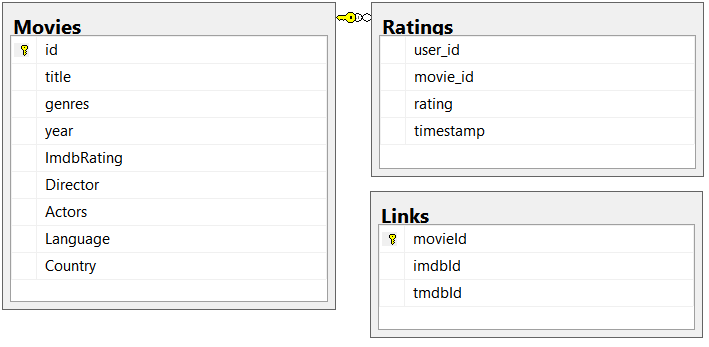
\includegraphics[width=1\textwidth]{movielens}
				\caption{Schemat bazy MovieLens}
				\label{fig:movielens_schema}
			\end{figure}
		
		\subsubsection{Yahoo Music}
		
			\todo{Opisać Yahoo Music}
		
		\subsubsection{Amazon Meta}
		
			\todo{Opisać Amazon Meta}
		
			\cite{leskovec2007dynamics}
		
	\section{Środowisko symulacyjne}
	
		\subsection{Oprogramowanie}
	
		Rys. \ref{fig:program} przedstawia zrzut ekranu środowiska symulacyjnego opracowanego przez autorkę pracy na potrzeby przeprowadzenia badań algorytmów. Główny interfejs programu składa się z trzech części: ustawienia podstawowe, okno z wynikiem oraz panel sterujący ustawieniami zaawansowanymi. 
	
		\begin{figure}[!ht] 
			\centering
			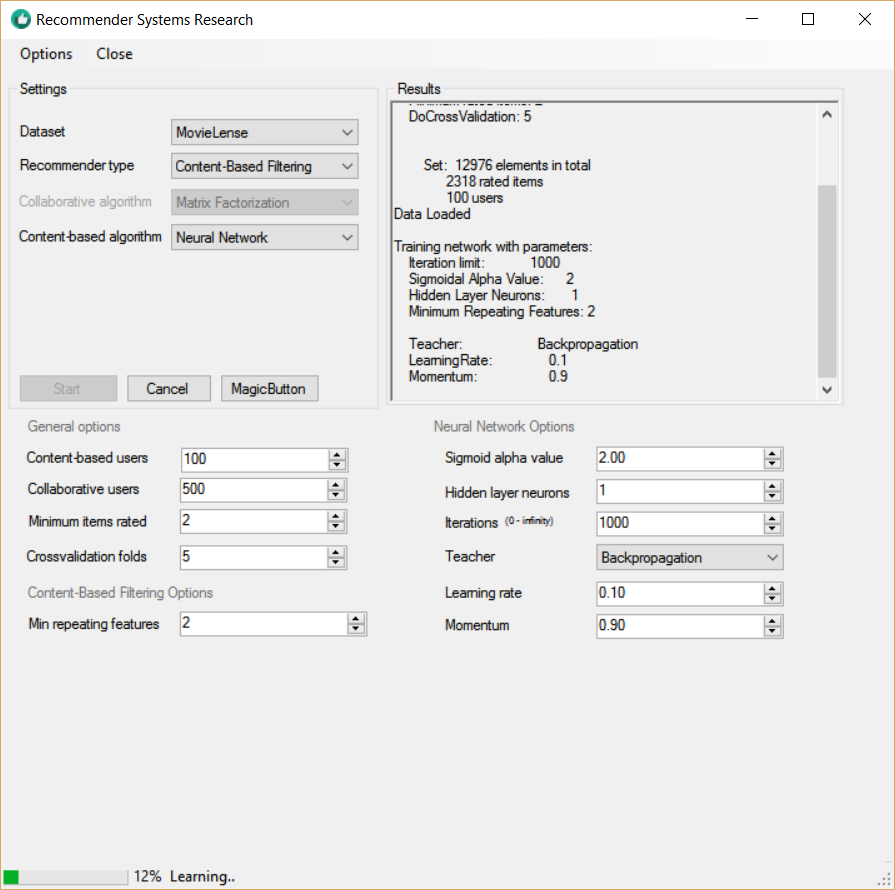
\includegraphics[width=1\textwidth]{program}
			\caption{Zrzut ekranu środowiska symulacyjnego}
			\label{fig:program}
		\end{figure}
	
		W sekcji z ustawieniami podstawowymi możliwy jest wybór:
		\begin{itemize}
			\item bazy danych, która zostanie wykorzystana do pomiarów;
			\item typu algorytmu rekomendującego (content-based, collaborative bądź hybrydowy)
			\item w przypadku wyboru kolaboratywnego filtrowania lub filtrowania hybrydowego możliwy jest wybór typu algorytmu: Matrix Factorization, Biased Matrix Factorization lub SVD++.
			\item w przypadku wyboru filtrowania z analizą zawartości lub filtrowania hybrydowego automatycznie wybierany jest algorytm oparty na sieci neuronowej. 
		\end{itemize}
		 
		 Widok ustawień zaawansowanych zmienia się w zależności od wybranego filtrowania. W przypadku wyboru content-based istnieje możliwość regulowania parametrów sieci neuronowej. Zawsze istnieje możliwość regulowania kryteriów doboru zestawu danych.
		 
		 Kryteria doboru zestawu danych są następujące:
		 
		 \begin{itemize}
		 	\item liczba użytkowników do pobrania do algorytmu content-based;
		 	\item liczba użytkowników do pobrania do algorytmu collaborative;
		 	\item minimum elementów, jakie zostały ocenione przez każdego pobranego użytkownika;
		 	\item stosunek wielkości zbioru treningowego do zbioru testowego (domyślnie 80\%-20\%).
		 \end{itemize}
		 
		 Parametry sieci neuronowej podlegające strojeniu to:
		 
		 \begin{itemize}
		 	\item Sigmoidalna wartość alfa; \todo{wcześniej powinien być zaprezentowany model sieci tak, żeby było wiadomo, skąd biorą się te parametry}
		 	\item liczba neuronów w warstwie ukrytej;
		 	\item maksymalna liczba iteracji uczenia sieci neuronowej;
		 	\item algorytm uczący sieć neuronową: propagacja wsteczna, rprop (resilient backpropagation) lub algorytm genetyczny;
		 	\item w przypadku wyboru algorytmu genetycznego -- rozmiar każdej kolejnej populacji;
		 	\item minimalna wymagana ilość powtórzeń danej cechy, aby była brana pod uwagę w trakcie budowania rekomendacji.
		 \end{itemize}	 
		
		\subsection{Sprzęt}
		
		Wszystkie badania zostały przeprowadzone na komputerze klasy PC działającym pod kontrolą 64--bitowego systemu Windows 10 Pro. Konfiguracja sprzętowa wygląda następująco:
		
		\begin{center}
			\begin{tabular}{ r  l  }
				Procesor: & Intel Core i5--6200U 2.30GHz \\ 
				RAM: & 8 GB \\  
				Typ dysku twardego: & SSD     
			\end{tabular}
		\end{center}
	
	\section{Przeprowadzone eksperymenty}
	
		\todo{Napisać tu ładny wstęp}
		\todo{Opis i schemat eksperymentów}
		\todo{?? Jak bardzo wchodzić w szczegóły?}
		
		Dla wszystkich przeprowadzonych eksperymentów stosunek zbioru treningowego do zbioru testowego wynosił 80\%/20\%.

		
		\subsection{Dopasowanie parametrów sieci neuronowej}
	
		Pierwszy przeprowadzony eksperyment miał na celu dopasowanie optymalnych parametrów sieci neuronowej dla filtrowania content-based. Badania przeprowadzone zostały w oparciu o bazę MovieLense. 
		
		\subsubsection{Dopasowanie maksymalnej liczby iteracji}
		\label{exp:expiterations}
		
			Uczenie sieci neuronowej odbywa się w pętli tak długo, jak wartość błędu na wyjściu spadnie poniżej określonej wartości bądź przekroczona zostanie maksymalna ilość iteracji. Eksperyment ma na celu zbadanie wartości błędów w zależności od liczby iteracji.
				
			\begin{center}
				\begin{longtable}{ | R{7cm}   m{8cm} |}
					\hline
					\multicolumn{2}{|c|}{\textbf{Konfiguracja parametrów podstawowych}} \\
					\hline
					Baza danych: & MovieLens \\
					Testowana metoda: & Content-based \\
					\hline
					\multicolumn{2}{|c|}{\textbf{Konfiguracja filtrowania content-based}} \\
					\hline
					Algorytm: & Sieć neuronowa uczona propagacją wsteczną, RPROP i algorytmem genetycznym \\
					Maksymalna ilość iteracji nauki: & ? \\				
					Ilość neuronów w warstwie ukrytej: & 1 \\
					Współczynnik momentum: & 0.9 \\
					Współczynnik uczenia: & 0.1 \\
					Sigmoidalna wartość $\alpha$: & 2.0 \\
					Minimum powtarzających się cech: & 10 \\
					Minimum ocenionych elementów przez użytkownika: & 10 \\
					Ilość testowanych użytkowników: & 10 \\				
					\hline
					\caption{Konfiguracja dla eksperymentu maksymalnej liczby iteracji}
				\end{longtable}
			\end{center}
			
			\todo{Zweryfikować, czy nie kłamię}
			Wyniki eksperymentu przedstawia wykres \ref{fig:expiterations} i tabela \ref{tab:expiterations}. Wraz ze wzrostem liczby iteracji wartość błędu maleje, jednakże po przekroczeniu pewnej wartości następuje ponowny wzrost. Wynika to z występowania zjawiska nadmiernego dopasowania (ang. \textit{overfitting}). 
			
			Zgodnie z oczekiwaniami, czas wykonania jest wprost proporcjonalny do liczby iteracji. W trakcie tego eksperymentu potwierdzone zostały również przypuszczenia dotyczące prędkości działania algorytmów. Najszybszy okazał się RPROP, jednakże kosztem nieco większych błędów. Najgorzej wypadł algorytm genetyczny, który charakteryzował się bardzo szybko rosnącym czasem wykonania przy jednoczesnym nie najlepszym wynikiem RMSE. 
			
			\begin{figure}[!ht]
				\centering
				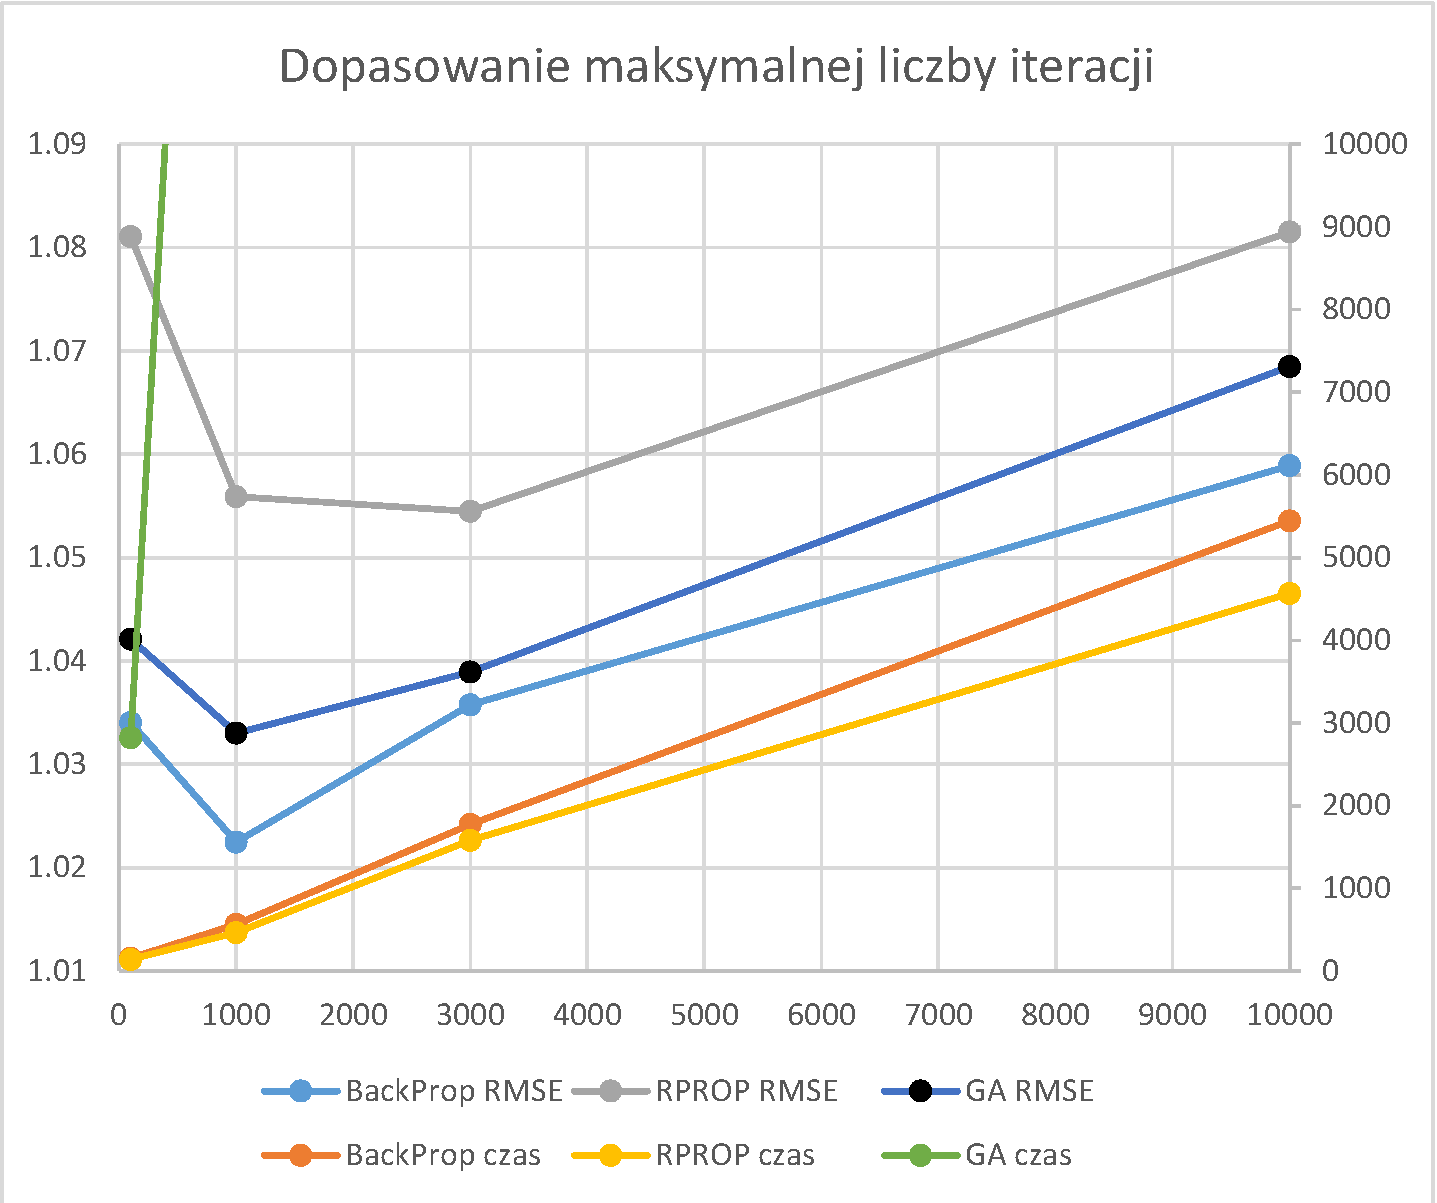
\includegraphics[width=0.7\textwidth]{expiterations}			
				\caption{Wyniki eksperymentu maksymalnej liczby iteracji}
				\label{fig:expiterations}
			\end{figure}
			

			\begin{longtable}{l||ll|ll|ll}		
				\label{tab:expiterations}		
				\textbf{L. iter.} & \multicolumn{2}{c|}{\textbf{Propagacja wsteczna}}  & \multicolumn{2}{c|}{\textbf{RPROP}} & \multicolumn{2}{c}{\textbf{Algorytm genetyczny}}  \\
				\hline
				& \textbf{RMSE} & \textbf{czas} & \textbf{RMSE} & \textbf{czas} & \textbf{RMSE} & \textbf{czas} \\
				\hline
				100 & 1.03402 & 155 & 1.081065 & 139 & 1.042103 & 2824 \\
				1000  & 1.022469 & 564 & 1.055915 & 463 & 1.033005 & 24831  \\
				3000  & 1.035766 & 1770 & 1.054472 & 1581  & 1.038922 & 70579  \\
				10000 & 1.058892  & 5444 & 1.081511  & 4567  & 1.068489 & 239775 \\
				\caption{Wyniki eksperymentu maksymalnej liczby iteracji}
			\end{longtable}
		
		\subsubsection{Dopasowanie parametru momentum} 
		\label{exp:momentum}
			
		Parametr momentum jest dodatkowym współczynnikiem mającym na celu ulepszenie działania algorytmu propagacji wstecznej (zob. \ref{sss:metoda_momentum}). Eksperyment ma na celu zbadanie dla jakich wartości osiągany jest najniższy błąd.
			
		\begin{center}
			\begin{longtable}{ | R{7cm}   m{8cm} |}
				\hline
				\multicolumn{2}{|c|}{\textbf{Konfiguracja parametrów podstawowych}} \\
				\hline
				Baza danych: & MovieLens \\
				Testowana metoda: & Content-based \\
				\hline
				\multicolumn{2}{|c|}{\textbf{Konfiguracja filtrowania content-based}} \\
				\hline
				Algorytm: & Sieć neuronowa z propagacją wsteczną \\
				Maksymalna ilość iteracji nauki: & 1000 \\				
				Ilość neuronów w warstwie ukrytej: & 2 \\
				Współczynnik momentum: & ? \\
				Współczynnik uczenia: & 0.1 \\
				Sigmoidalna wartość $\alpha$: & 2.0 \\
				Minimum powtarzających się cech: & 10 \\
				Minimum ocenionych elementów przez użytkownika: & 100 \\
				Ilość testowanych użytkowników: & 5 \\				
				\hline
				\caption{Konfiguracja dla eksperymentu dopasowania wartości momentum}
			\end{longtable}
		\end{center}
		
		Wyniki eksperymentu przedstawia wykres \ref{fig:expmomentum} i tabela \ref{tab:expmomentum}. W zakresie wartości $[0,0.9]$ błąd oscyluje w granicach podobnych wartości z nieznaczną tendencją malejącą. Wyraźny skok na niekorzyść odnotowany jest dopiero przy momentum$=1$. 
		
		\begin{figure}[!ht]
			\centering
			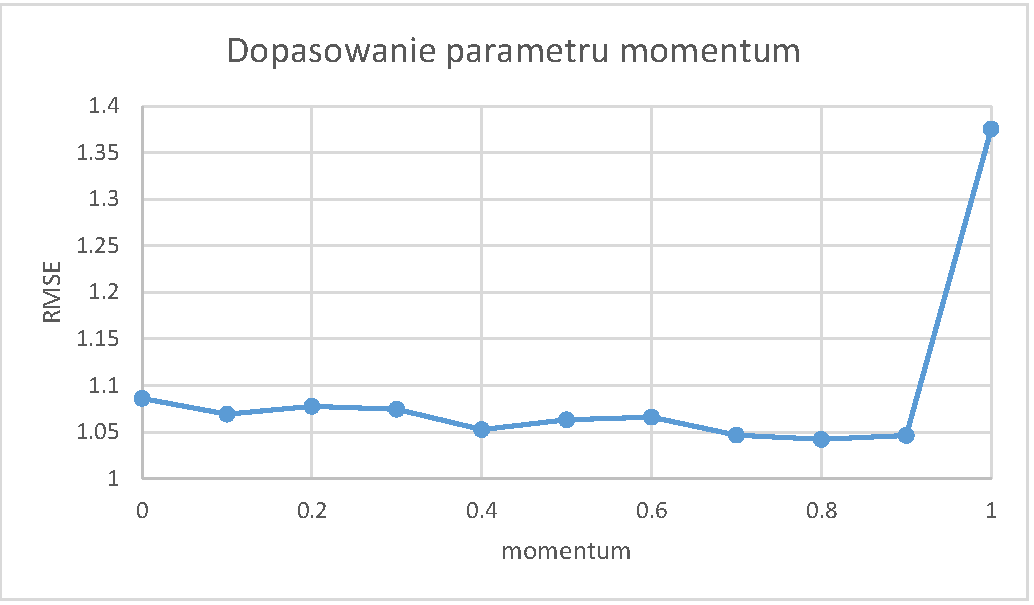
\includegraphics[width=0.7\textwidth]{expmomentum}			
			\caption{Wyniki eksperymentu momentum}
			\label{fig:expmomentum}
		\end{figure}
				
		\begin{longtable}{lll}
			\label{tab:expmomentum}
			\textbf{Momentum} & \textbf{RMSE} & \textbf{MAE} \\
			\hline
			0        & 1.086007 & 0.855964 \\
			0.1      & 1.069125 & 0.851345 \\
			0.2      & 1.077596 & 0.860146 \\
			0.3      & 1.074588 & 0.851467 \\
			0.4      & 1.052529 & 0.8424   \\
			0.5      & 1.063205 & 0.846198 \\
			0.6      & 1.065994 & 0.856964 \\
			0.7      & 1.046752 & 0.83462  \\
			0.8      & 1.042235 & 0.842353 \\
			0.9      & 1.046243 & 0.840319 \\
			1        & 1.375336 & 1.071652 \\
			\caption{Wyniki eksperymentu momentum}
		\end{longtable}
					
		\subsubsection{Dopasowanie rozmiaru populacji}
	
		Parametr rozmiaru populacji determinuje ilość osobników, jaka zostanie wygenerowana w każdej epoce przebiegu algorytmu genetycznego (zob \ref{ss:algorytm_genetyczny}). Eksperyment ma na celu zbadanie korelacji pomiędzy rozmiarem populacji a błędem algorytmu rekomendacji. Mierzony jest również czas uczenia sieci neuronowej.
		
		\begin{center}
			\begin{longtable}{ | R{7cm}   m{8cm} |}
				\hline
				\multicolumn{2}{|c|}{\textbf{Konfiguracja parametrów podstawowych}} \\
				\hline
				Baza danych: & MovieLens \\
				Testowana metoda: & Content-based \\
				\hline
				\multicolumn{2}{|c|}{\textbf{Konfiguracja filtrowania content-based}} \\
				\hline
				Algorytm: & Sieć neuronowa uczona algorytmem genetycznym \\
				Maksymalna ilość iteracji nauki: & 1000 \\				
				Ilość neuronów w warstwie ukrytej: & 1 \\
				Współczynnik momentum: & 0.9 \\
				Współczynnik uczenia: & 0.1 \\
				Sigmoidalna wartość $\alpha$: & 2.0 \\
				Minimum powtarzających się cech: & 10 \\
				Minimum ocenionych elementów przez użytkownika: & 10 \\
				Ilość testowanych użytkowników: & 10 \\				
				\hline
				\caption{Konfiguracja dla eksperymentu dopasowania wielkości populacji}
			\end{longtable}
		\end{center}
		
		Wyniki eksperymentu przedstawia wykres \ref{fig:exppopulation} i tabela \ref{tab:exppopulation}. Zgodnie z oczekiwaniami występuje dodatnia korelacja pomiędzy rozmiarem populacji a czasem wykonania i ujemna pomiędzy rozmiarem populacji a błędem algorytmu rekomendacji. 
		
		Zależność pomiędzy rozmiarem populacji a czasem wykonania  jest liniowa, natomiast błąd maleje wykładniczo gdy populacja osiąga większe rozmiary. Optymalnym zatem jest przyjęcie rozmiaru populacji równej $100$. 
		
		
		\begin{figure}[!ht]
			\centering
			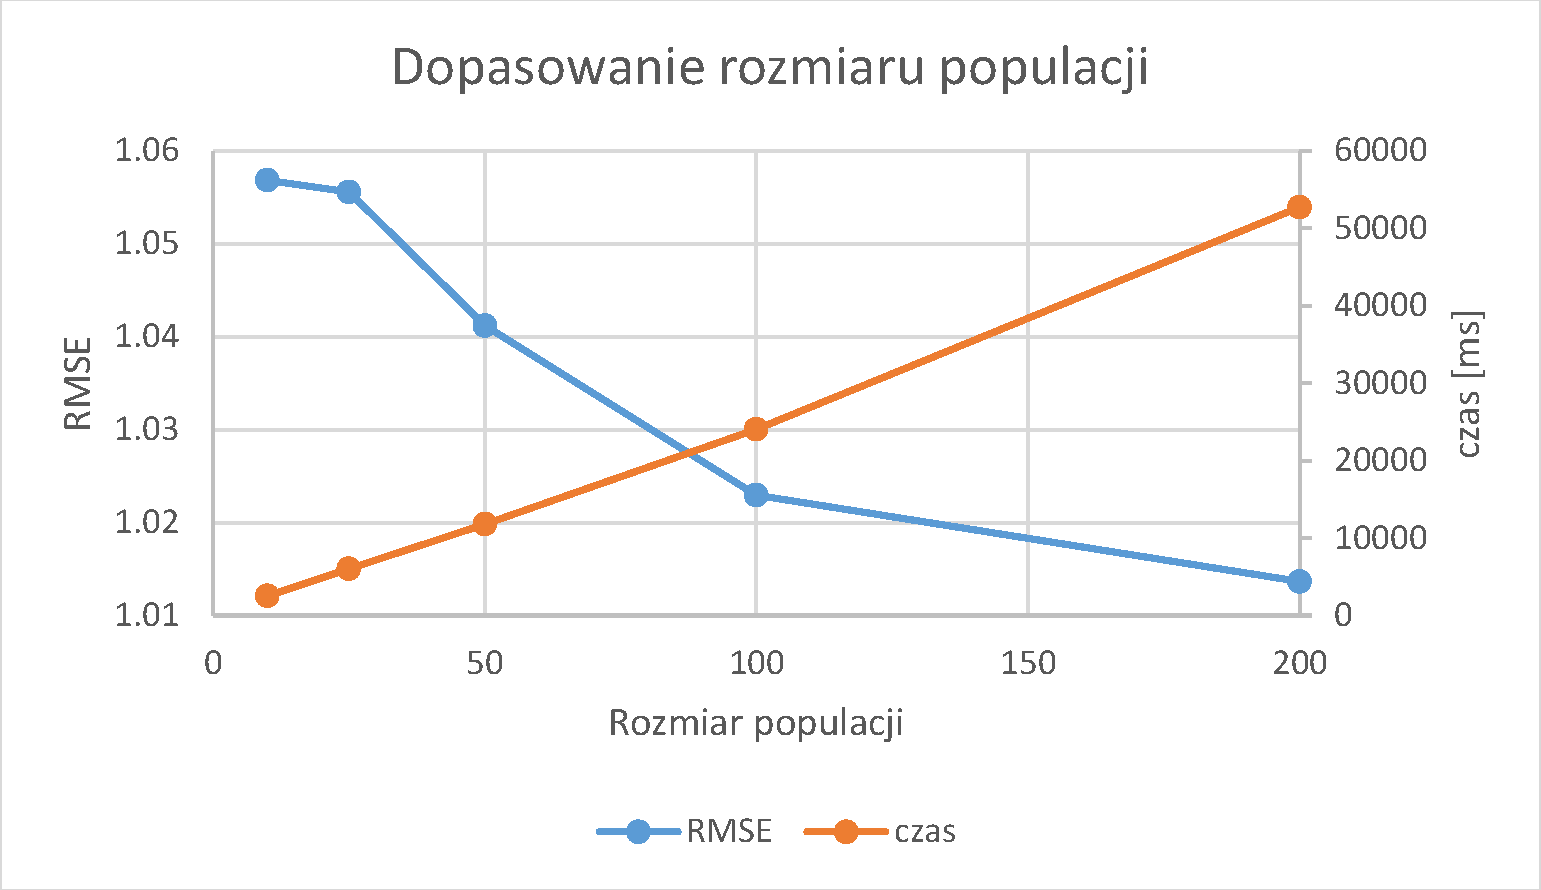
\includegraphics[width=0.7\textwidth]{exppopulation}
			\caption{Wyniki eksperymentu rozmiaru populacji}
			\label{fig:exppopulation}
		\end{figure}
		
		\begin{longtable}{llll}
			\label{tab:exppopulation}
			\centering
			\textbf{Populacja} & \textbf{RMSE} & \textbf{MAE} & \textbf{czas} \\
			\hline
			10        & 1.056848 & 0.861325 & 2519                      \\
			25        & 1.055562 & 0.859391 & 6015                      \\
			50        & 1.041198 & 0.850866 & 11804                     \\
			100       & 1.022943 & 0.825477 & \multicolumn{1}{r}{24062} \\
			200       & 1.013656 & 0.816789 & 52751                     \\
			\caption{Wyniki eksperymentu rozmiaru populacji}
		\end{longtable}
	

		
		\subsubsection{Dopasowanie ilości neuronów w warstwie ukrytej}
		
			\todo{Koniecznie TODO}
		
		\subsubsection{Dopasowanie współczynnika uczenia}
		
			\todo{Czy trzeba?}
		
		\subsubsection{Dopasowanie wartości alfa}
		
			\todo{Czy trzeba}

		\subsection{Porównanie algorytmu hybrydowego z content-based i collaborative}

			\todo{Porównanie algorytmu hybrydowego z content-based i collaborative}

		\subsection{Analiza statystyczna wyników}		\todo{Analiza statystyczna wyników, PQStat}

\chapter{Wnioski}
\shortTitle{Wnioski}

	\todo{Wnioski}

\chapter{CHAPTER 1}
\section{SECTION}

\def\alghoritm4{Alghoritm 4}
\begin{algorithm}
\caption{\alghoritm4}
\myalgorithm{\alghoritm4}
\label{aq:algStat}
\begin{algorithmic}
\STATE $T \leftarrow \text{text under analysis}$
\FOR{each word $w \in T$}
    \STATE $S_{w}\leftarrow FIND\_SENTIMENT(w) $
    \IF {$S_{w}=POSITIVE$}
        \STATE $Sentiment[POSITIVE]++$
    \ELSIF{$S_{w}=NEGATIVE$}
        \STATE $Sentiment[NEGATIVE]++$
    \ELSE 
        \STATE $Sentiment[NEUTRAL]++$
    \ENDIF
\ENDFOR
%\STATE $x\in\{POSITIVE,NEGATIVE,NEUTRAL\}$
\RETURN $\arg\max_x Sentiment[x]$
\end{algorithmic}
\end{algorithm}


\def\schema1{Schema 1}
\begin{figure}[ht]
\caption{\schema1}
\myfigure{\schema1}
\label{fig:kdb}
\begin{center}
    <GRAPHIC>
\end{center}
\end{figure}

\section{Section 2}

\subsection{Subsection 1}

\subsubsection{Subsubsection 1}

\begin{mydef}
\textbf{Definicja} - pierwsza
\end{mydef}



 \clearpage
\appendix
\chapter{Appendix 1}


\clearpage
\pagestyle{plain}
\listofmyfigure
\listofmyequations
\listofmyalgorithm
\clearpage

%\{apalike}%Used BibTeX style is unsrt

\bibliographystyle{iisthesis}
\bibliography{bibliography}

\end{document}

